\documentclass{report}
\author{Ben Haladik}
\title{Bioinformatische Anwendung von \textit{Graphlets} zur Analyse von Proteinstrukturtopologien zur Analyse von Proteinen \\ Rohfassung}
\usepackage{mathtools}
\usepackage{amsfonts}
\usepackage{ngerman}
\usepackage{hyperref}
%\usepackage{natbib}
\usepackage{rotating}
\usepackage[table, dvipsnames, usenames]{xcolor}
\usepackage{color}
\usepackage[justification=centering]{caption}
%\usepackage{algorithm2e}
%\usepackage{qtree}
%\usepackage{cite}
\definecolor{fGreen}{rgb}{0.13,0.54,0.13}

\begin{document}

\definecolor{green}{rgb}{0.13,0.54,0.13}


\maketitle

\newpage

\tableofcontents

\newpage

\chapter{Einleitung}

\section{Motivation}

TODO: Zitationen einf\"ugen: schwierigkeit der Analyse, bereits bekannte Methoden
TODO: stärkerer Bezug auf und nennung von tatianas arbeit (insbesondere bio-graphlets)
TODO: Bereits bekannte Anwendungen von Graphlets: Anwendung von Shervashidze auf ZUSAMMENHAENGENDE graphen, zeigt Probleme mit der Darstellung in der PTGL - einzelne Knoten werden nur in marginaler Weise integriert.
Anwendung von Przulj: Grosse Netzwerke . Vergleich mit zufaelligen Graphen. Vergleich zwischen PPIs mit hoher Praezision und PPIs mit niedriger praezision. betrifft ebenfalls nur vollstaendige graphen.
datensatz von dobson und doig (in shervashidze arbeit erwaehnt) verwendet svms zur analyse - 70 prozent genauigkeit wurde erreicht. dies ist ein anzeichen daf\"ur, dass die Klassifizierung mit vektoren nur begrenzt genutzt werden kann. (shervashidze ergebnis ist auch nicht viel besser)
es ist zu erw\"ahnen, dass SVMs zu den fortgeschrittensten Klassifizierungsmethoden geh\"oren, die zur zeit verwendet werden.


\paragraph{Proteine} sind gewisserma"sen die Wekzeuge der Zelle. Fast jede Aufgabe die sie bew\"altigen muss, um zu \"uberleben, l\"ost sie mit Hilfe von Proteinen. Dementsprechend vielf\"altig sind die Formen und Funktionen, die Proteine annehmen - und wie bei Werkzeugen auch, folgt die Form der Funktion. Die Aufkl\"arung der dreidimensionalen Struktur von Proteinen ist somit f\"ur ein tiefergehendes Verst\"andnis ihrer Funktion von zentraler Bedeutung.



Im Rahmen der \textit{•}




\paragraph{\textit{Graphlets}} sind kleine vollst\"andige induzierte Teilgraphen.






\section{\textit{State of the Art}}

TODO: Methoden nennen, weitere Zitationen

Es gibt bereits einige Methoden, um Proteinstrukturen miteinander zu vergleichen. \textit{Hasegawa et al} \cite{advancespitfalls} liefern einen umfangreichen Vergleich verschiedener Methoden, bei denen Strukturen auf unterschiedlichen Abstraktionsstufen betrachtet und verglichen werden. So k\"onnen Proteinstrukturen dreidimensional, zweidimensional und eindimensional betrachtet und verglichen werden.

\paragraph{3D-Methoden} versuchen zun\"achst mittels Sequenzalignment einen Bereich in den zu vergleichenden Proteinen zu finden, in dem sich beide Proteine sehr \"ahnlich sind. Dieser Bereich fungiert gewisserma"sen als \emph{Anker} f\"ur das weitere Alignment. In den weiteren Schritten werden die Proteine so positioniert, dass die Distanzen in dem alignierten Bereich minimal sind. Von diesem \textit{Template} ausgehend, werden die Distanzen zwischen den weiteren Residuen der Proteine berechnet und meist mittels \textit{Root-mean-square-deviation} bewertet.

\paragraph{2D-methoden} versuchen Kontakte zwischen Residuen oder Sekund\"arstrukturen zu vergleichen. Diese Kontakte werden beispielsweise als graphen oder Distanzmatrizen dargestellt. Der Vergleich zwischen zwei Proteinstrukturen wird dann beispielsweise als Verlgeich zweier Distanzmatrizen durchgef\"uhrt.

\paragraph{1D-Methoden} nutzen Strukturprofile zur Darstellung von Proteinen. In Strukturprofilen repr\"asentieren einzelne Buchstaben Eigenschaften von Residuen und die Konformation des Protein-\textit{Backbone} an der entsprechenden Stelle. So k\"onnen schnelle \textit{String}-Algorithmen genutzt werden, um Strukturen zu suchen und zu vergleichen.

\paragraph{0D-Methoden} reduzieren die 3D-Struktur am st\"arksten. Die gesamte Struktur wird durch eine Zahl beschrieben, die sich aus der Struktur berechnen l\"asst. Sie erlauben sehr schnelle Suchen in Datenbanken, haben aber das Problem, dass sie keinen Vergleich von Teilstrukturen erm\"oglichen.

\paragraph{Die Methoden} stellen alle einen Versuch dar, die \"Ahnlichkeit von Proteinen zu beziffern. Sie werden angewendet, um entferent homologe Proteine aufzusp\"uren und in Datenbanken eine \"Ahnlichkeitssuche zu erm\"oglichen. Dies findet vor allem im pharmakologischen Bereich Anwendung.

Interessant ist, dass unter den von \textit{Hasegawa et al} vorgestellten 1D-Methoden keine wirklich analog zur Analyse mit \textit{Graphlets} funktioniert. Andere 1D-Methoden versuchen die Polypeptidkette als \textit{String} darzustellen und damit die Konformations\"anderung des \textit{Backbone} zu beschreiben. Im Gegensatz dazu z\"ahlt der \textit{Graphlet}-Algorithmus die \textit{Graphlets} unabh\"angig von ihrer Position im Graphen. Somit repr\"asentiert der \textit{Graphlet}-Vektor an jeder Stelle eine globale Eigenschaft des Graphen, anstatt die Ver\"anderung von einer Sekund\"arstruktur zur n\"achsten zu beschreiben.

Des weiteren sind die meisten Methoden, die Proteinstrukturen vergleichen, \textit{Template}-basiert. Um den Suchraum einzuschr\"anken muss eine Struktur ausgew\"ahlt werden, die als Vorlage f\"ur den Vergleich mit anderen Strukturen dient. Dementsprechend \"andert sich das Ergebnis des Vergleichs auch in Abh\"angigkeit der gew\"ahlten Vorlage.



\section{Ziele}

Ziel dieser Arbeit war zun\"achst die Erweiterung der Funktionalit\"at des \texttt{graphletAnalyser}. Hierzu geh\"ort eine funktionierende Datenbankanbindung, so dass die \textit{Graphlet}-Vektoren f\"ur alle verschiedenen Graphtypen korrekt in die PTGL eingetragen werden k\"onnen.
Die Suche nach markierten \textit{Graphlets} sollte so implementiert werden, dass sie auf Graphen mit beliebigen Markierungen angewandt werden kann. Deshalb wurde ein Algorithmus entwickelt und implementiert, der aus einem Alphabet von Knotenmarkierungen alle Worte berechnet, die markierte  2- und 3-\textit{Graphlets} repr\"asentieren - der \textit{Graphlet}-Worte-Algorithmus.
Schlussendlich sollte im durch Fallstudien \"uberpr\"uft werden, ob und inwiefern sich \textit{Graphlets} eignen, um die \"Ahnlichkeit von Proteinstrukturtopologien zu untersuchen. Dies wurde mit unterschiedlichen Metriken getestet.

\section{Aufbau der Arbeit}

Zun\"achst wird im Kapitel \emph{Materialien und Methoden} PLCC vorgestellt - das Programm, mit dem die Graphen der PTGL erzeugt werden.
Es folgt eine Kurzbeschreibung der PTGL selbst, sowie eine Beschreibung des \textit{Graphlet}-Algorithmus und des \textit{Graphlet}-Worte-Algorithmus.
Weiterhin wird das Programm \texttt{graphletAnalyser}vorgestellt, welches den \textit{Graphlet}-Algorithmus implementiert.
Anschlie"send werden verschiedene Metriken vorgestellt, mit denen die erhaltenen \textit{Graphlet}-Vektoren verglichen werden.
Die Ergebnisse dieses Vergleichs werden im Teil Ergebnisse und Diskussion vorgestellt. Hierbei werden die verschiedenen Metriken verglichen und es wird \"uberpr\"uft inwiefern die Suche nach markierten \textit{Graphlets} zu diesem Ergebnis beitr\"agt.

\chapter{Materialien und Methoden}

Um die Proteinstrukturtopologien aus der PTGL zu vergleichen wurde das Programm \texttt{graphletAnalyser} genutzt und erweitert. Es wurde bereits 2013 von \textit{Tatiana Bakirova} im Rahmen ihrer Diplomarbeit im Arbeitskreis \textit{Molekulare Bioinformatik} geschrieben. Die urspr\"ungliche Funktionalität wurde erweitert. Hierbei wurden Funktionen zur Analyse von Komplexgraphen, Aminos\"auregraphen und den Sekund\"arstrukturgraphen implemetiert. Diese Graphen stammen allesamt aus der PTGL (\underline{P}rotein \underline{T}opology \underline{G}raph \underline{L}ibrary) von Tim Sch\"afer.


\section{Die PTGL}


Die \underline{P}rotein \underline{T}opology \underline{G}raph \underline{L}ibrary ist 2009 von \textit{May et al.} \cite{ptgl1} entwickelt worden. Ausgehend von der Tatsache, dass sich Proteinstrukturtopologien als r\"aunliche Beziehungen von SSEs untereinander definieren lassen, verwendet die PTGL \emph{Graphen}, um Proteinstrukturtopologien darzustellen.
Hierbei stellen die Knoten des Graphen die SSEs eines Proteins dar. Sie werden dem jeweiligen SSE entsprechend markiert. Knoten, die $\alpha$-Helices repr\"asentieren werden mit einem H markiert, $\beta$-Faltbl\"atter mit einem E. Weiterhin erm\"oglicht die PTGL die Darstellung von Liganden, (\cite{vplg}) denen mit L markierte Knoten zugeordnet werden. Um die r\"aumliche Nachbarschaft von Sekund\"arstrukturen und Liganden untereinander darstellen zu k\"onnen werden ungerichtete Kanten zwischen Knoten gezogen wenn die entsprechenden Elemente benachbart sind. Jede Polypeptidkette eines Proteins wird dann als \emph{Proteingraph} dargestellt. Die Zusammenhangskomponenten eines Proteingraphen werden als Faltungsgraphen bezeichnet, weil sie typischerweise eine unabh\"angige Faltungseinheit darstellen.

\paragraph{Die Berechnung dieser Graphen}

erfolgt unter Verwendung der entsprechenden PDB und DSSP Dateien. Um den Graphen einer Polypeptidkette zu berechnen werden aus der DSSP-Datei die Sekund\"arstrukturelemente (SSEs) des Proteins ausgelesen. F\"ur jedes Paar von SSEs wird die Anzahl der r\"aumlichen Kontakte ihrere Residuen berechnet. Wenn die Anzahl dieser Kontakte einen gewissen Grenzwert \"uberschreitet, wird die angenommen, dass diese SSEs r\"aumlich benachbart sind und die jeweiligen Knoten werden durch eine Kante verbunden.

\paragraph{Komplexgraphen}

werden ebenfalls in dieser Arbeit untersucht. Ihre Berechnung erfolgt analog zur Berechnung der Proteingraphen. Komplexgraphen k\"onnen einen vollst\"andigen Proteinkomplex darstellen. In einem solchen Graphen werden zus\"atzlich die Nachbarschaften von SSEs unterschiedlicher Polypeptidketten einbezoogen. Ein Komplexgraph setzt sich also aus mehreren Proteingraphen zusammen. Hier wird jedem Knoten zus\"atzlich zum SSE die Zugeh\"origkeit zu einer Polypeptidkette zugeordnet.

\paragraph{Aminos\"auregraphen} werden ebenfalls untersucht und analog zu Proteingraphen berechnet. Hier werden keine SSEs betrachtet. Stattdessen repr\"asentiert jeder Knoten eine Aminos\"aure eines Proteins. Die Knoten werden entsprechend der chemischen Eigenschaften der Aminos\"auren markiert. Knoten, die saure oder basische Residuen darstellen werden mit einem c markiert. Ein p markiert Knoten f\"ur polare Residuen, die weder sauer noch basisch sind. F\"ur unpolare Aminos\"auren wird ein h verwendet. Auch Liganden k\"onnen in Aminos\"auregraphen dargestellt werden. Ihre Knoten werden durch ein ? markiert.


F\"ur die Berechnungen dieser Arbeit wurde eine lokale Datenbank erstellt, die das gleiche Schema wie die PTGL verwendet.

\section{Der \textit{Graphlet}-Algorithmus}





\paragraph{Motivation}
Die PTGL \cite{vplg} erm\"oglicht also die Darstellung von Proteinstrukturtopologien als Graphen. Um aus diesen Graphen weitere Informationen zu gewinnen, ist es sinnvoll, sie untereinander vergleichen zu k\"onnen. Ein solcher Vergleich ist jedoch ein schwieriges Problem: Gesucht ist eine Funktion $f: (G,G') \rightarrow \mathbb{R} $, die f\"ur zwei Graphen $G$ und $G'$ deren \"Ahnlichkeit zueinander beziffert.
Es gibt diverse M\"oglichkeiten diesesd Problem zu bearbeiten, von denen jedoch keine einfach ist.
Eine M\"oglichkeit ist, die Suche nach gr\"o"sten gemeinsamen isomorphen Teilgraphen in $G$ und $G'$, oder man versucht eine Editierdistanz zu berechnen - also herauszufinden, wie viele Operationen (Hinzuf\"ugen oder Entfernen von Knoten und Kanten) n\"otig sind um $G$ in $G'$ zu \"uberf\"uhren. Diese beiden genannten Methoden erfordern jedoch aufw\"andige Berechnungen.
Deshalb werden Methoden verwendet, die \emph{Topologische Charakteristiken} berechnen und dies in polynomieller Laufzeit bewerkstelligen. Der Vorteil hierbei ist, dass die (aufw\"andige) Berechnung dieser Charakteristiken nur einmal pro Graph erfolgen muss. Die Charakteristika k\"onnen dann als Vektoren verglichen werden und man spart sich die Berechnungen, die man sonst f\"ur alle Paare von Graphen $G,G'$ durchf\"uhren muss.



\paragraph{Beschreibung des Algorithmus}
\textit{Graphlets} sind kleine induzierte Teilgraphen eines gr\"o"seren ungerichteten Graphen. \textit{N. Shervashidze} stellte diese Methode als Vergleichsschema f\"ur Graphen 2009 zum ersten Mal vor.  (Literaturverweis einf\"ugen). Folgendes Bild zeigt alle \textit{Graphlets} der Gr\"o"se 4:

\begin{figure}[h]
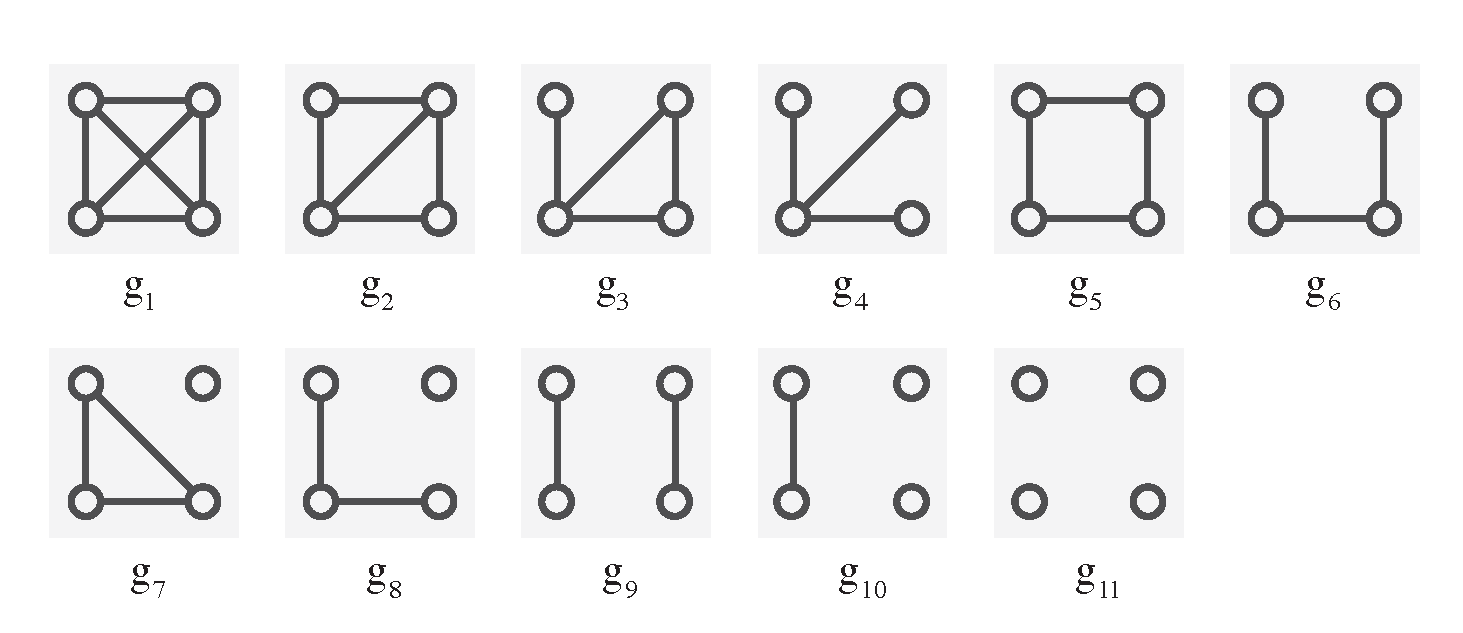
\includegraphics[width =\linewidth]{4graphlets.pdf}
\caption{Graphlets der Gr\"o"se 4 (\textit{Shervashidze et al.})}
\label{fig:4graphlets}
\end{figure}


Um ein \textit{Graphlet} der Gr\"o"se k zu finden, besucht der Algorithmus alle Euler-Wege der L\"ange k, in dem gegebenen Graphen. F\"ur jeden dieser Wege \"uperpr\"uft er, f\"ur alle Paare von Knoten $v,w$ ob es eine Kante $e = {v,w}$ gibt, die nicht zu dem besuchten Euler-Weges gehg\"ort. Je nachdem, welche Kanten hierbei gefunden werden, wird der Z\"ahler f\"ur das entsprechende \textit{Graphlet} erh\"oht. Der Algorithmus z\"ahlt hier aber nur alle zusammenh\"angenden \textit{Graphlets}. Er verwendet die folgenden Gewichtungsvektoren: 


\begin{subequations}
\label{eq:w-vector}
\textit{Graphlet}-Gewichtungsvektoren
\begin{align}
w_2 := \left( \frac{1}{2} \right) \\
w_3 := \left( \frac{1}{6}, \frac{1}{2} \right) \\
w_4 := \left( \frac{1}{24}, \frac{1}{12}, \frac{1}{4}, 1, \frac{1}{8},\frac{1}{2} \right) \\
w_5 := \left( \frac{1}{120}, \frac{1}{72}, \frac{1}{48}, \frac{1}{36}, \frac{1}{28}, \frac{1}{20}, \frac{1}{14}, \frac{1}{10}, \frac{1}{12}, \frac{1}{8}, \frac{1}{4}, \frac{1}{2}, \frac{1}{12} \frac{1}{12}, \frac{1}{4} \frac{1}{4}, \frac{1}{2}, 1, \frac{1}{2}, 1\right)
\end{align}
\end{subequations}

Jede Stelle eines Vektors $w_i$ ist mit einem \textit{Graphlet} assoziiert. Da der Algorithmus alle Euler-Wege einer L\"ange $i$ in dem Graphen abl\"auft, sind in den Vektoren Br\"uche eingetragen, wobei der Z\"ahler f\"ur die Anzahl der Euler-Wege der L\"ange $i$ steht. Dies stimmt nat\"urlich nicht f\"ur die sogenannten Stern-\textit{Graphlets} ($g_4$ in \ref{fig:4graphlets} $g_{19}$,$g_{20}$ und $g_{21}$ in \ref{fig:5graphlets}). Da diese keinen Euler-Weg der L\"ange 4 bzw. 5 enthalten werden sie anders gez\"ahlt.
(beispiel mit Pseudocode einf\"ugen?)

\subsection{Der \textit{Graphlet}-Worte-Algorithmus}

In der letzten Version von \texttt{graphletAnalyser} war es bereits m\"oglich markierte \textit{Graphlets} mit 2 und 3 Knoten in Proteingraphen zu z\"ahlen. Diese Funktionalit\"at wurde im Rahmen dieser Arbeit verallgemeinert, so dass der Nutzer beliebige Alphabete angeben kann.
Der Algorithmus erh\"alt das Alphabet $\sum = \{ \sigma_i : i \in \mathbb{N} \}$ der Knotenmarkierungen. Aus diesem Alphabet berechnet er Worte $w$, die zur Repr\"asentation der markierten \textit{Graphlets} genutzt werden.
Hierbei k\"onnen verschiedene Worte das gleiche \textit{Graphlet} repr\"asentieren. Im Falle von 2-\textit{Graphlets} repr\"asentieren die zwei Worte $(\sigma_i,\sigma_j)$ und $(\sigma_j, \sigma_i)$ das gleiche markierte \textit{Graphlet} mit den Knotenmarkierungen $\sigma_i,\sigma_j$. Worte, die das gleiche \textit{Graphlet} repr\"asentieren, werden im Folgenden als \emph{\"aquivalente Graphlet-Worte}  bezeichnet.


Die Berechnung der \"aquivalenten \textit{Graphlet}-Worte der L\"ange 2 ist trivial. Aus dem Alphabet $\sum$ werden alle Worte $w = (\sigma_i, \sigma_j)$ berechnet, wobei Spiegelungen nicht mit ausgegeben werden, da zwei Worte $ (\sigma_j, \sigma_i) $ und $ (\sigma_j, \sigma_i) $ \"aquivalente \textit{Graphlet}-Worte sind.

Die Berechnung aller \"aquivalenten \textit{Graphlet}-Worte der L\"ange 3 ist komplizierter, da sie f\"ur zwei verschiedene \textit{Graphlets} berechnet werden m\"ussen. F\"ur das \textit{Graphlet} $g_1$ sind alle Worte \"aquivalent zueinander, die zyklische Vertauschungen voneinander sind. F\"ur das \textit{Graphlet} $g_2$ sind Worte \"aquivalent zueinander, die Spiegelungen voneinander sind (siehe Abbildung \ref{fig:3graphlets}). \\



%\begin{algorithmic}
% INPUT: Ein Alphabet \sum = \{ \sigma_1, ... , \sigma_n \}
% OUTPUT: Zwei Listen Wortliste_3-Weg, Wortliste_3-Kreis \sub \sum*
% Liste Wortliste_3-Weg
% Liste Wortliste_3-Kreis
%\For{ i = 1 to n}
% Wortliste.add(\sigma_i \sigma_i \sigma_i)
%\For{ k = i + 1 to n}
% Wortliste_3-Weg.add(\sigma_i \sigma_k \sigma_i)
% Wortliste_3-Weg.add(\sigma_i \sigma_i \sigma_k)
% Wortliste_3-Weg.add(\sigma_i \sigma_k \sigma_k)
% Wortliste_3-Weg.add(\sigma_k \sigma_i \sigma_k)
%
% Wortliste_3-Kreis.add(\sigma_i \sigma_k \sigma_i)
% Wortliste_3-Kreis.add(\sigma_i \sigma_k \sigma_k)
%\For{ m = k + 1 to n}
% Wortliste_3-Weg.add(\sigma_i \sigma_k \sigma_m)
% Wortliste_3-Weg.add(\sigma_m \sigma_i \sigma_k)
% Wortliste_3-Weg.add(\sigma_k \sigma_m \sigma_i)
%
% Wortliste_3-Kreis.add(\sigma_i \sigma_k \sigma_m)
% Wortliste_3-Kreis.add(\sigma_m \sigma_k \sigma_i)
%\EndFor
%\EndFor
%\EndFor
%\end{algorithmic}

Pseudocode Platzhalter \\
Pseudocode Platzhalter \\
Pseudocode Platzhalter \\
Pseudocode Platzhalter \\
Pseudocode Platzhalter \\
Pseudocode Platzhalter \\
Pseudocode PLatzhalter \\
Pseudocode PLatzhalter \\
Pseudocode PLatzhalter \\
Pseudocode PLatzhalter \\
Pseudocode PLatzhalter \\
Pseudocode PLatzhalter \\
Pseudocode PLatzhalter \\
Pseudocode PLatzhalter \\
Pseudocode PLatzhalter \\
Pseudocode PLatzhalter \\
Pseudocode PLatzhalter \\
Pseudocode PLatzhalter \\
Pseudocode PLatzhalter \\
Pseudocode PLatzhalter \\
Pseudocode PLatzhalter \\
Pseudocode PLatzhalter \\
Pseudocode PLatzhalter \\


Der Algorithmus besteht aus 3 \textit{for}-Schleifen, die \"uber das Alphabet iterieren. In der \"au"sersten Schleife werden Worte hinzugef\"ugt, in denen alle Buchstaben gleich sind.
In der zweiten Schleife wird jeweils der n\"achste Buchstabe des Alphabets betrachtet. F\"ur jedes Paar $a, b$ von Buchstaben \"uber einem Alphabet $\sum$ sind die Mengen der \"aquivalenten Worte f\"ur das \textit{Graphlet} $g_1$ $P_{3-Kreis} = \{ \}$ und $P_{3-Weg} = \{ aaa, aba, aab, abb  \}$ f\"ur das \textit{Graphlet} $g_2$

TODO: Beschreibung der Mengen, Beweis



F\"ur das Alphabet der SSE- und Komplexgraphen $ \sum_{SSE} := \{ H, E, L \} $ und das Alphabet der Aminos\"auregraphen $ \sum_{AA} := \{ h, p, c, ? \} $ gibt der oben beschriebene Algorithmus die folgenden Listen aus:


\begin{subequations}
\begin{align}
p_2 := (HH, HE, HL, EE, EL, LL) \\
p_{3-Weg} := (HHH, HEH, HHE, HEE, EHE, HEL, LHE, ELH, HLH, HHL, HLL, LHL, EEE, ELE, EEL, ELL, LEL, LLL) \\
p_{3-Kreis} := (HHH, HEH, HEE, HEL, LEH, HLH, HLL, EEE, ELE, ELL, LLL) \\
\end{align}
\end{subequations}

Die Vektoren $a_2, a_{3-Weg}$ und $a_{3-Kreis}$ beschreiben die Worte f\"ur \textit{Graphlets} in AA-Graphen 

\begin{subequations}
\begin{align}
a_2 := (hh, hp, ha, h?, pp, pa, p?, aa, a?, ??) \\
a_{3-Weg} := (hhh, hph, hhp, hpp, php, hpa, ahp, pah, hp?, ?hp, p?h, hah, hha, haa, aha, ha?, ?ha ,a?h, h?h, hh?, h??, ?h?, ppp, pap, ppa, paa, apa, pa?, ?pa, a?p, p?p, pp?, p??, ?p?, aaa, a?a, aa?, a??, ?a?, ???) \\
a_{3-Kreis} := (hhh, hph, hpp, hpa, aph, hp?, ?ph, hah, haa, ha?, ?ah, h?h, h??, ppp, pap, paa, pa?, ?ap, p?p, p??, aaa, a?a, a??, ???)
\end{align}
\end{subequations}




\section{\texttt{graphletAnalyser}}

Das Programm \texttt{graphletAnalyser} implementiert die oben beschriebenen Algorithmen und kann die Resultate der Berechnungen in verschiedenen Formaten lokal auf dem Rechner des Nutzers speichern und sie in einer \textit{Postgresql}-Datenbank ablegen, die mit PLCC erstellt wurde.
\texttt{graphletAnalyser} ist in C++ geschrieben und nutzt die \textit{Boost-Graph-Library} zur internen Darstellung der Graphen.

Das Programm wird \"uber die Konsole gestartet und erh\"alt als \textit{Input} eine oder mehrere GML-Dateien. Der Nutzer kann weiterhin \"uber Parameter festlegen, ob markierte \textit{Graphlets} berechnet werden sollen, ob die Resultate in einer mit PLCC erstellten Datenbank gespeichert werden sollen und ob er die vordefinierten Knotenmarkierungen von SSE-Graphen, Komplexgraphen oder Aminos\"auregraphen nutzen m\"ochte.

Weiterhin k\"onnen in der Konfigurationsdatei nutzerdefinierte Alphabete von Knotenmarkierungen eingegeben werden, die bei der Berechnung markierter \textit{Graphlets} genutzt werden k\"onnen.


Das Programm bestand bereits vor dem Beginn dieser Arbeit. Es wurden Fehler im Code beseitigt und einige Funktionen hinzugef\"ugt, die im folgenden kurz beschrieben werden. 

\paragraph{Das Einlesen von Komplexgraphen und Aminos\"auregraphen}

ist implementiert worden. Die entsprechenden Alphabete sind im Programmcode vordefiniert und k\"onnen vom Nutzer \"uber Parameter ausgew\"ahlt werden.

\paragraph{Nutzerdefinierte Knotenmarkierungen} k\"onnen nun in der Konfigurationsdatei angegeben werden. Der Nutzer kann ein Alphabet von Knotenmarkierungen und ein \textit{Label} unter dem diese Knotenmarkierungen in den GML-Dateien abgelegt sind angeben. F\"ur dieses Alphabet werden alle \"aquivalenten \textit{Graphlet}-Worte durch den \textit{Graphlet}-Worte-Algorithmus berechnet. Diese werden dann bei der Berechnung der markierten \textit{Graphlets} im Graphen unter dem vorgegebenen \textit{Label} gesucht und gez\"ahlt.
Es k\"onnen also beliebige Alphabete und \textit{Labels} angegeben werden, so lange die Markierungen der Knoten nicht mehr als einen Buchstaben enthalten. 
 

\paragraph{Die Datenbankanbindung} wurde um Funktionen zum Speichern von Aminos\"auregraphen und Komplexgraphen erweitert. Das Speichern von Vektoren markierter \textit{Graphlets} wurde implementiert.



\section{Scoring}





\subsection{Relative \textit{Graphlet}-H\"aufigkeiten-Distanz}

\textit{N. Pr\v{z}ulj et al.} haben \textit{Graphlets} bereits in verschiedensten Zusammenh\"anen auf biologische Daten wie Protein-Protein-Interaktionsnetzwerke \cite{frqdistribution} angewandt. Als Ma"s f\"ur die \"Ahnlichkeit von Netzwerken nutzen sie die Relative-\textit{Graphlet}-H\"aufigkeiten-Distanz (RGF) $D(G,H)$. Diese Metrik berechnet den Abstand zwischen zwei Graphen $G$ und $H$ als logarithmierte Differenz der normalisierten Anzahl der \textit{Graphlets} in $G$ und $H$. Sie ist folgenderma"sen definiert: \\

Sei $N_{i}(G)$ die Anzahl der \textit{Graphlets} von Typ $i \in {1,...,29}$ und \\ $T(G) = \sum_{i = 1}^{29} N_{i}(G)$ die Anzahl der \textit{Graphlets} in $G$, beziehungsweise $H$\\

Dann ist die Relative-\textit{Graphlet}-H\"aufigkeiten-Distanz $D(G,H)$ f\"ur zwei Graphen $G$ und $H$ definert als:

\begin{subequations}
\begin{align}
D(G,H) := \sum_{i = 1}^{29} | F_{i}(G) - F_{i}(H) | \\
mit F_{i}(G) := - log(\frac{N_{i}(G)}{T(G)})
\end{align}
\end{subequations}



Diese Metrik l\"asst sich analog zur euklidischen Distanz, oder einer beliebigen anderen Vektornorm auffassen, denn sie berechnet f\"ur jeden Index $i$ die Differenz zwischen den Stellen $x_i,y_i$ zweier Vektoren $x$ und $y$. Sie verwendet die normalisierten \textit{Graphlet}-Vektoren unter der Annahme, dass die \"Ahnlichkeit zweier Netzwerke sich aus der \"Ahnlichkeit lokaler Substrukturen ableiten l\"asst \cite{frqdistribution}. Somit k\"onnen Netzwerke, die \"ahnliche Substrukturen habe, sich aber in ihrer Gr\"o"se stark unterschieden, immer noch als \"ahnlich erkannt werden.
Weiterhin wurde gezeigt, \cite{frqdistribution} dass diese Metrik auch bei verrauschten Daten noch sehr gut funktioniert. Hierbei ist jedoch zu beachten, dass sie bisher vor allem f\"ur sehr gro"se Netzwerke mit mehreren Tausend Knoten und Kanten verwendet wurde. Diese Gr\"o"se kann von Aminos\"auregraphen erreicht werden, wenn sie gro"se Proteine modellieren. Proteingraphen und Komplexgraphen sind aber deutlich kleiner.


\subsection{Modifizierter Jaccard-Index}

Der Jaccard-Index ist im eigentlichen Sinne ein Ma"s, um die \"Ahnlichkeit von gleichm\"achtigen Mengen zu bewerten. F\"ur zwei Mengen $A,B$ berechnet sich der Jaccard-Index $D_{Jac}(A,B)$ folgenderma"sen:

\[ D_{Jac}(A,B) := \frac{\sum_{x \ in A \land x \in B} 1}{\sum_{x \in A \lor x \in B} 1} \]

Dementsprechend sind zwei Mengen $A,B$ gleich, wenn  gilt $D_{Jac} = 1$ und disjunkt, wenn gilt $D_{Jac} = 0$. Mit ihm wird die relative Anzahl der Elemente beider Mengen berechnet.
Um dieses Ma"s in sinnvoller Weise auf \textit{Graphlet}-Vektoren zu \"ubertragen wurde ein zus\"atzlicher Faktor $k \in \mathbb{R} $ mit $k \in [0,1]$  eingef\"uhrt, der als Pr\"azisionsfaktor zu verstehen ist. Die Defintion des modifizierten Jaccard-Index $D_{Jac-m}(v,w)$ f\"ur zwei Vektoren $v,w$ lautet also:

\[ D_{Jac-m}(v,w) := \frac{\sum_{i = 1}^n x_i}{\sum_{x \in A \lor x \in B} 1} \]

Hierbei gilt:

\[ x_i = 
   \begin{cases}
     1     & \quad \mathrm{if} \quad v_i >= w_i \times k \land w_i >= v_i \times k \\
     0     & \quad \mathrm{else} \\
   \end{cases}
\]

In dieser modifizierten Variante werden zwei Vektoren $v,w$ als gleich angesehen, wenn sich $v_i,w_i$ f\"ur alle $i$ h\"ochstens um den Faktor $k$ unterschieden.
Dies steht im Gegensatz zur RGF, die - analog zu einer Vektornorm - die Abst\"ande zwischen zwei \textit{Graphlet}-Vektoren misst.



\section{Datens\"atze}


\subsection{Fallstudien - Datensatz 1}

Anfangs wurden 20 verschiedene Proteine aus verschiedenen CATH-Klassen zum Vergleich ausgew\"ahlt. Die Proteine wurden so gew\"ahlt, dass die drei CATH-klassen mit vielen Sekund\"arstrukturelementen \textit{mainly-alpha}, \textit{mainly-beta} und \textit{alpha-beta} vertreten sind. Weiterhin wurde die Auswahl so getroffen, dass es f\"ur jede Stufe der Hierarchie mindestens zwei Proteine gibt, die auf der entsprechenden Stufe in die gleiche Klasse eingeordnet werden. Die Proteine werden im folgenden kurz beschreiben.


\subsubsection{4-Helix-\textit{Bundles}}

Das Cytochrom B562 von \emph{E. coli} (Bild einf\"ugen) ist ein Protein, das f\"ur Elektronentransport zust\"andig ist. Strukturell wird es als 4-Helix-\textit{Bundle} eingeordnet. Zu diesem Protein gibt es zwei PDB-Eintr\"age: 1QPU und 256B. Es gibt von diesem Protein auch eine Hem-bindende Variante, die oxidiert ist. Sie hat die PDB-ID 1QQ3. All diese Strukturdaten werden von CATH als sehr \"ahnliche Strukturen mit hoher Sequenzidentit\"at eingeordnet.
Um die Parameter und Metriken f\"ur den Vergleich zu testen, bietet es sich an, diese Proteine mit weiteren Proteinen aus der selben homologen Superfamilie zu vergleichen und diese dann mit Proteinen aus anderen Homologen Superfamilien zu vergleichen. Die entsprechenden Proteine werden h\"andisch entsprechend der Einordnung durch CATH gew\"ahlt. Proteine die neu designt wurden k\"onnten sich auch anbieten. Inwiefern eine Untersuchung an ihnen sinnvoll ist, muss aber noch \"uberpr\"uft werden.
Weitere Proteine aus der Homologen Superfamilie, die sich eignen sind:\\
2XL6: Cytochrom C aus Alcaligenes Xylosoxidans, gebunden mit NO\\
2YL1: s.o. nur andere Variante mit anderem Bindungspartner.\\
Diese beiden m\"ussten strukturell \"ahnlicher sein, als die weiter oben genannten Varianten von Cytochrom B562.\\
Die oben genannten Proteine werden von CATH alle in die \emph{Topologie} der 4-Helix-\textit{Bundles} (Hemerythrin Untereinheit A) eingeordnet. Sie sind alle Teil der selben homologen Superfamilie.

Zum Vergleich werden weiterhin 1rxq und 2qe9 aus der Homologen Superfamilie \textit{dinb family like domain}  




\subsubsection{Wachstumshormone}

Sie k\"onnen mit Proteinen aus der Topologie \textit{Growth Hormone, Chain A} verglichen werden. Denn beide werden von CATH in die gleiche Architektur \emph{Up-down bundle} eingeordnet. Proteine aus dieser Topologie sind: \\
1HGU: Menschliches Wachstumshormon\\
1M4R: Rekombinantes menschliches Interleukin 22\\
1D9C: Rinder Interferon Gamma \\
Die oben genannten Proteine aus der Topologie der Wachstumshormone haben eine Sequenzidentit\"at zwischen 35 und 60 Prozent. Sie scheinen sich gut f\"ur die untersuchung zu eignen.
Das Protein mit der PDB-ID 1PV6 liegt in der selben Topologie, wird aber in eine andere Superfamilie eingeordnet.

\subsubsection{Aldolasen}

Die Aldolasen 7TIM, 1NEY und 2V5L werden durch das gleich Gen in Hefe codiert. Da sie eine $\beta$-\textit{Barrel}-Struktur besitzen, sollten sie eine niedrigere \textit{Graphlet}-Distanz zueinander aufweisen, als zu allen anderen Strukturen.

\subsubsection{Zusammengefasst}

\begin{tabular}{l r}

PDB-ID & CATH-Code  \\
2UTG & 1.10.210.10  \\ % uteroglobin - pdb-klasse: steroid bindend
1VIB & 1.10.287.120 \\ % neurotoxin - pdb-klasse: neurotoxin
1QPU & 1.20.120.10  \\ % Cytochrom b
1QQ3 & 1.20.120.10  \\ % cytochrom b oxidiert
2XL6 & 1.20.120.10  \\ % cytochrom c mit NO
2YL1 & 1.20.120.10  \\ % cytochrom c mit CO
1rxq & 1.20.120.450 \\ % metall abhaengige hydrolase - pdb-head: metall abhaengiges protein
2qe9 & 1.20.120.450 \\ % metall abhaengige hydrolase - pdb-head: hydrolase
2RD9 & 1.20.120.450 \\ % metall abhaengige hydrolase - pdb-head: hydrolase
1M4R & 1.20.1250.10 \\ % interleukin 22 - pdb-head: cytokin
1HGU & 1.20.1250.10 \\ % wachstumshormon - pdb-head: hormon
1PV6 & 1.20.1250.20 \\ % lactose permease - pdb-head: transportprotein
1AWR & 2.40.100.10  \\ % enzymkomplex cypa und hagpia ?
1D9C & 1.20.1250.10 \\ % BOVINE INTERFERON-GAMMA
1NGL & 2.40.128.20  \\ % transportprotein
1N7V & 2.105.10.10  \\ % riesiges Virusprotein - rezeptor bindendes protein
7TIM & 3.20.20.70   \\ % triosephosphat isomerase phosphat-komplex
1NEY & 3.20.20.70   \\ % triosephosphat isomerase DHAP-komplex
2V5L & 3.20.20.70   \\ %  TRYPANOSOMAL TRIOSEPHOSPHATE ISOMERASE - neue kristallform
1V3Z & 3.30.70.100  \\ % Acylphosphatase
1A17 & 1.25.40.10   \\ % pdb-header sagt hydrolase - muesste anderen hydrolasen aehnlich sein
1ar0 & 3.10.450.50  \\ % Nuclear transport factor 2

\end{tabular}


\subsection{Fallstudien  - Datensatz 2} 

F\"ur die ersten Tests wurden verschiedene Proteine entsprechend ihrer CATH-Klassifizeirungen zusammengestellt. Die Proteine wurden so gew\"ahlt, dass die 3 CATH-Klassen gleich stark vertreten sind, in denen sich viele Sekund\"arstrukturelemente befinden. Dementsprechend wurden Proteine aus der CATH-Klasse 4 ignoriert. Diese Klasse enth\"alt nur Proteine mit wenigen Sekund\"arstrukturelementen.

Es befinden sich je 5 Vertreter der drei CATH-Klassen 1 (\textit{mainly-alpha}), 2 (\textit{mainly-beta}) und 3 (\textit{alpha-beta}) in diesem Datensatz. Diese wurden so gew\"ahlt, dass je ein Paar innerhalb der selben Klasse ein direkter struktureller Nachbar mit eine Sequenzidentit\"at von mehr als 95\%, sowie ein Nachbar mit einer Sequenzidentit\"at von meher als 35\% befindet, um zu \"uberpr\"ufen, ob die \textit{Graphlet}-Vektoren von Aminos\"auregraphen eine Korrelation mit der Sequenzidentit\"at aufweisen k\"onnen.
Weiterhin wurde je ein Vertreter der selben Topologie aus einer anderen Superfamilie, sowie der selben Architektur mit anderer Topologie gew\"ahlt.
 
Da die \textit{Graphlet}-Vektoren globale Eigenschaften eines Graphen beschreiben, wurde bei diesem Datensatz darauf geachtet, dass alle Strukturen aus genau einer Polypeptidkette mit genau einer Dom\"ane bestehen.

Diese Herangehensweise folgt aus der Vermutung, dass einzelne Dom\"anen charakteristische \textit{Graphlet}-Vektoren haben. 
\\

\begin{tabular}{ | c || c | c |}

\hline
PDB-ID & CATH-ID        & Klassifizierung      \\ \hline
1qpu   & 1.20.120.10 & Elektronentransport     \\ \hline
1qq3   & 1.20.120.10 & Elektronentransport     \\ \hline
1cgn   & 1.20.120.10 & Elektronentransport     \\ \hline
1he9   & 1.20.120.260& Toxin (Exoenzym)        \\ \hline
3gf9   & 1.20.900.10 & Endocytose              \\ \hline
1exs   & 2.40.128.20 & Lipid bindendes Protein \\ \hline
1ngl   & 2.40.128.20 & Transport Protein       \\ \hline
1qqs   & 2.40.128.20 & Zucker bindendes Protein\\ \hline
3slo   & 2.40.128.130& Protein Transport       \\ \hline
1wjx   & 2.40.280.10 & RNA-bindendes Protein   \\ \hline
5chy   & 3.40.50.2300& Signaltransduktion      \\ \hline
2id9   & 3.40.50.2300& Signal Protein          \\ \hline
3i42   & 3.40.50.2300& unbekannte Funktion     \\ \hline
1d4o   & 3.40.50.1220& Oxidoreductase          \\ \hline
2w0i   & 3.40.20.10  & Transferase             \\ 
\hline
\end{tabular}



\subsubsection{Vergleich von Proteinen \"ahnlicher Gr\"o"se}

Da \textit{Graphlets} in den Experimenten von Pruzlj et al und Shervashidze et auf gro"se Graphen angewandt wurden, bietet es sich an, sie auch auf gro"se Proteinkomplexe anzuwenden und bei kleinen Proeinen den Aminsos\"auregraphen zu verwenden. So kann man (hoffentlich) das Problem der d\"unn besetzten Graphen umgehen und f\"ur verschiedene Gr\"o"sen von Graphen relevante Ergebnisse erzielen. Daf\"ur muss ein Datensatz aus gr\"o"sen Proteinkomplexen mit bekannter struktureller \"Ahnlichkeit zusammengestellt werden.



\subsection{Fallstudien - Datensatz 3}



\chapter{Ergebnisse}

\section{Fallstudien - Datensatz 1}

Die paarweisen RGF-Distanzen der Proteine befinden sich in den Tabellen \ref{table:occ-pg-rgf} \ref{table:occ-aag-rgf} und \ref{table:occ-cg-tc}. Die paarweisen Jaccard-Indizes befinden sich in den Tabellen \ref{table:occ-aa-tc}, \ref{table:occ-pg-tf} und \ref{table:occ-cg-tc}.
Hierbei wurden die Zellen, die die 4 besten Bewertungen f\"ur das Protein der entsprechenden Zeile enthalten gr\"un eingef\"arbt. Hierbei gilt, dass das Gr\"un umso dunkler ist, je st\"arker die \"Ahnlichkeit bewertet wird.

\paragraph{Der Vergleich mittels RGF}
zeigt f\"ur die Aminos\"auregraphen die st\"arksten \"Ahnlichkeiten immer innerhalb der entsprechenden CATH-Klassen. Sowohl die Proteine aus der \textit{mainly-alpha}-Klasse, als auch die Proteine der \textit{mainly-beta}-Klasse haben die besten \"Ahnlichkeitswerte mit Proteinen der gleichen Klasse.
Innerhalb der Klasse der \textit{alpha-beta}-Proteine, gibt es mit 2id9 und 1d4o zwei Proteine, denen eine gr\"o"sere \"Ahnlichkeit zu Proteinen der \textit{mainly-alpha}-Klasse attestiert wurde.
Bei 1d4o f\"allt auf, dass der niedrigste Wert mit 7,091 deutlich h\"oher ist, als die besten Werte aller anderen Proteine.
2id9 hat laut der RGF-Distanz die gr\"o"ste \"Ahnlichkeit zu 1he9.
Bis auf diese beiden Au"snahmen l\"asst sich jedoch eine gro"se starke Korrelation mit den CATH-Klassen erkennen.
Alle anderen Proteine haben mindestens die zwei kleinsten zwei RGF-Distanzen zu Vertretern aus der selben CATH-Klasse.

Dies gilt f\"ur die Aminos\"auregraphen. Die RGF-Distanzen der Proteingraphen zueinander zeigen ein weniger klares Bild.
F\"ur die \textit{mainly-alpha}-Klasse und die der \textit{mainly-beta}-Klasse befinden sich die Proteine mit den k\"urzesten Distanzen immer noch in der selben Klasse. Dies l\"asst sich f\"ur die Proteine der \textit{alpha-beta}-Klasse aber nicht mehr behaupten. Hier haben 2ID9, 3I42 und 2w0I die k\"urzesten Distanzen zu Proteinen anderer Klassen.

Bei den Komplexgraphen ist die Korrelation zwischen der RGF-Distanz und der Zugeh\"origkeit zur CATH-Klasse noch geringer. Die Tabelle \ref{table:occ-cg-rgf} zeigt nur f\"ur die Proteine 1QQ3, 1HE9, 1EXS und 1QQS die k\"urzeste Distanz zu einem Vertreter der gleichen Klasse.
Es f\"allt jedoch auf, dass besonders h\"aufig die Proteine der \textit{alpha-beta}-Klasse 5CHY, 2ID9 und 3I42 als \"ahnlich zu anderen bewertet werden.

\paragraph{Der Vergleich der Jaccard-Indizes}
zeigt ein \"ahnliches Bild, wie der Vergleich der RGF-Distanzen. Bei den Aminos\"auregraphen zeigt sich, dass innerhalb der \textit{mainly-alpha}-Klasse wieder die paarweisen \"Ahnlichkeiten der \textit{mainly-alpha}-Proteine am gr\"o"sten sind. Dies gilt bis auf eine Ausnahme auch f\"ur die \textit{mainly-beta}-Proteine. Das Protein mit der PDB-ID 1NGL wird als strukturell \"ahnlichstes Protein zu 2W0I bewertet. In der Klasse der \textit{alpha-beta}-Proteine gibt es mit 2ID9 und 1D4O wieder zwei Ausrei"ser, die die gr\"o"sten paarweisen \"Ahnlichkeiten nicht zu Vertretern der eigenen Klasse haben. F\"ur 2ID9 wird 1HE9 als \"ahnlichstes Protein angegeben und 1D4O wird 1QQS zugeordnet.

Die paarweisen Tanimoto-Koeffizienten der Proteingraphen zeigen - wie schon bei den RGF-Distanzen - eine geringere Korrelation mit der Zugeh\"origkeit zu den CATH-Klassen, als die Koeffizienten der Aminos\"auregraphen. Es haben zwar wieder mindestens 3 Vertreter jeder Klasse ihren n\"achsten Nachbarn in der gleichen Klasse, aber es gibt auch einige Proteine, die ihren n\"achsten Nachbarn au"serhalb der eigenen Klasse haben. Hierzu geh\"oren 1D4O, 2W0I (beide \textit{alpha-beta}) und 3GF9 (\textit{mainly-alpha}). Es f\"allt auf, dass wieder die Proteine mit den PDB-DIs 2ID9 und 3I42 besonders h\"aufig als strukturell \"ahnlich zu vielen anderen Proteinen bewertet werden.

F\"ur die Komplexgraphen zeigt die Tabelle wieder eine hohe \"Ahnlichkeite unter den ersten 3 Proteinen 1QPU, 1QQ3 und 1CGN. Auch innerhalb der Klasse \textit{alpha-beta} sind 3 Proteine mit der h\"ochsten paarweisen \"Ahnlichkeit bewertet worden. Die geringe Anzahl von stark bewerteten \"Ahnlichkeiten innerhalb der \textit{mainly-beta}-Klasse ist sehr auff\"allig. 1QQS und 3SLO sind das einzige Paar mit \textit{beta}-Topologie, dessen \"Ahnlichkeit als gro"s bewertet wurde.

\section{Fallstudien - Datensatz 2}

\section{Fallstudien - Datensatz 3}


\chapter{Diskussion und Ausblick}



\section{Diskussion}

Die folgende Diskussion der Fallstudien widmet sich vor allem der Frage, wieso die Ergebnisse der \"Ahnlichkeitsvergleiche, sich so stark zwischen den jeweiligen Graphendarstellungen unterscheiden.
Des weiteren wird der Zusammenhang zwischen dem Jaccard-Index und der RGF untersucht.

\subsection{Datensatz 1}

Wie schon im Ergebnisteil dargestellt, zeigen die Vergleiche der Aminos\"auregraphen den h\"ohsten Konsens mit der Einteilung der Strukturen durch CATH und SCOPe. Eine m\"ogliche Erkl\"arung hierf\"ur ist die Gestalt der Graphen. Bisher wurden \textit{Graphlets} haupts\"achlich zur Analyse von zusammenh\"angenden Graphen verwendet (\cite{sherv_graphlets}, \cite{graphletfrequency}).
Proteingraphen und Komplexgraphen sind jedoch nicht immer zusammenh\"angend. es kommt h\"aufig vor, dass einzelne Knoten keine Verbindungen zum Rest des Graphen aufweisen. Das unten stehende Bild zeigt ein Beispiel.

\begin{figure}[h!]
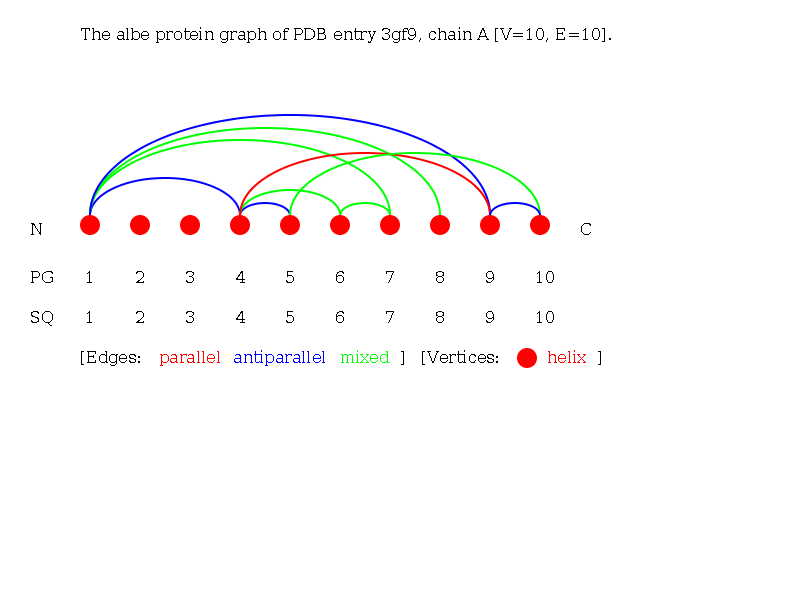
\includegraphics[scale=0.5]{3gf9_A_albe_PG.png}
\caption{Proteingraph von 3GF9 - Datensatz 1}
\end{figure}

Dadurch, dass dies in den zusammenh\"angenden \textit{Graphlets} nicht ber\"ucksichtigt werden kann, geht Information verloren. Unabh\"angig von der Wahl des \"Ahnlichkeitsma"s w\"urde dieser Graph mit einem anderen Graphen, dem die beiden Helix-Knoten mit einem Grad von 0 fehlen, als gleich bewertet werden, obwohl dieser zwei SSEs weniger aufwiese. Diese SSEs k\"onnen jedoch biologisch von zentraler Bedeutung sein.

Im Gegensatz hierzu sind die Aminos\"auregraphen dieser Fallstudie zusammenh\"angend. Dies erkl\"art die h\"ohere Genauigkeit. 



\subsection{Datensatz 2}

\subsection{Datensatz 3}

\section{Ausblick}

\subsection{Verbesserung des Scoring}

\subsection{Optimierung der Laufzeit von \texttt{graphletAnalyser}}

\subsection{\"Ahnlichkeitssuche}

\subsection{\textit{Graphlets} im Faltungsraum}

\subsection{\textit{Graphlet}-Motive}





\chapter{Anhang}


\section{Bildverzeichnis}

\begin{figure}[h!]
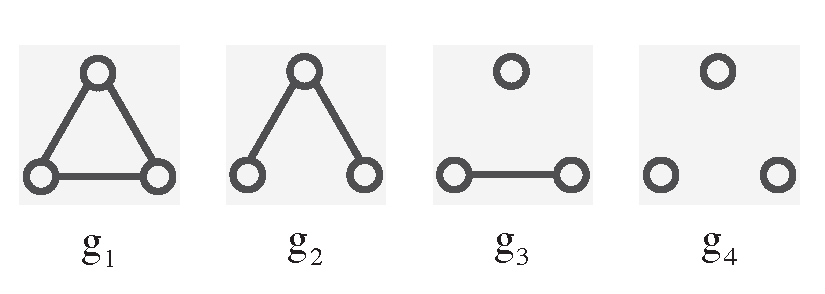
\includegraphics[width =\linewidth]{3graphlets.pdf}
\caption{Graphlets der Gr\"o"se 3 (\textit{Shervashidze et al.})}
\label{fig:3graphlets}
\end{figure}

\begin{figure}[h!]
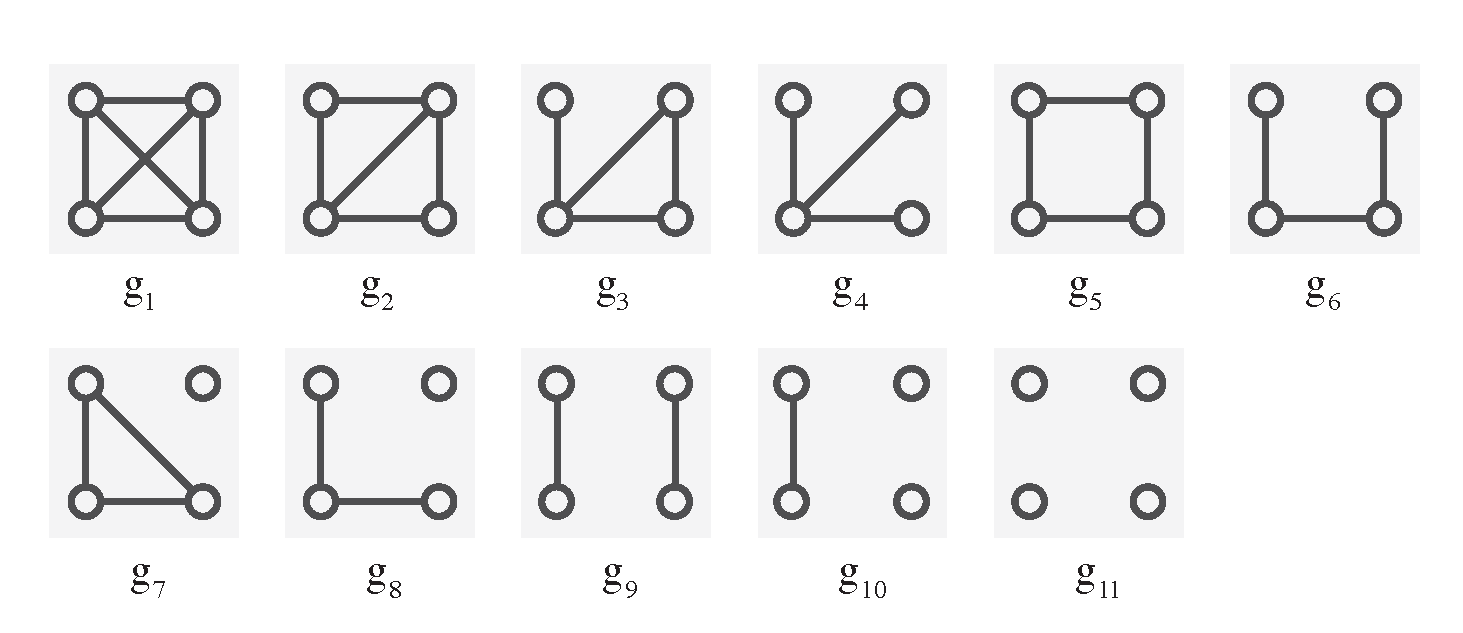
\includegraphics[width =\linewidth]{4graphlets.pdf}
\caption{Graphlets der Gr\"o"se 4 (\textit{Shervashidze et al.})}
\label{fig:4graphlets2}
\end{figure}

\newpage

\begin{figure}[h!]
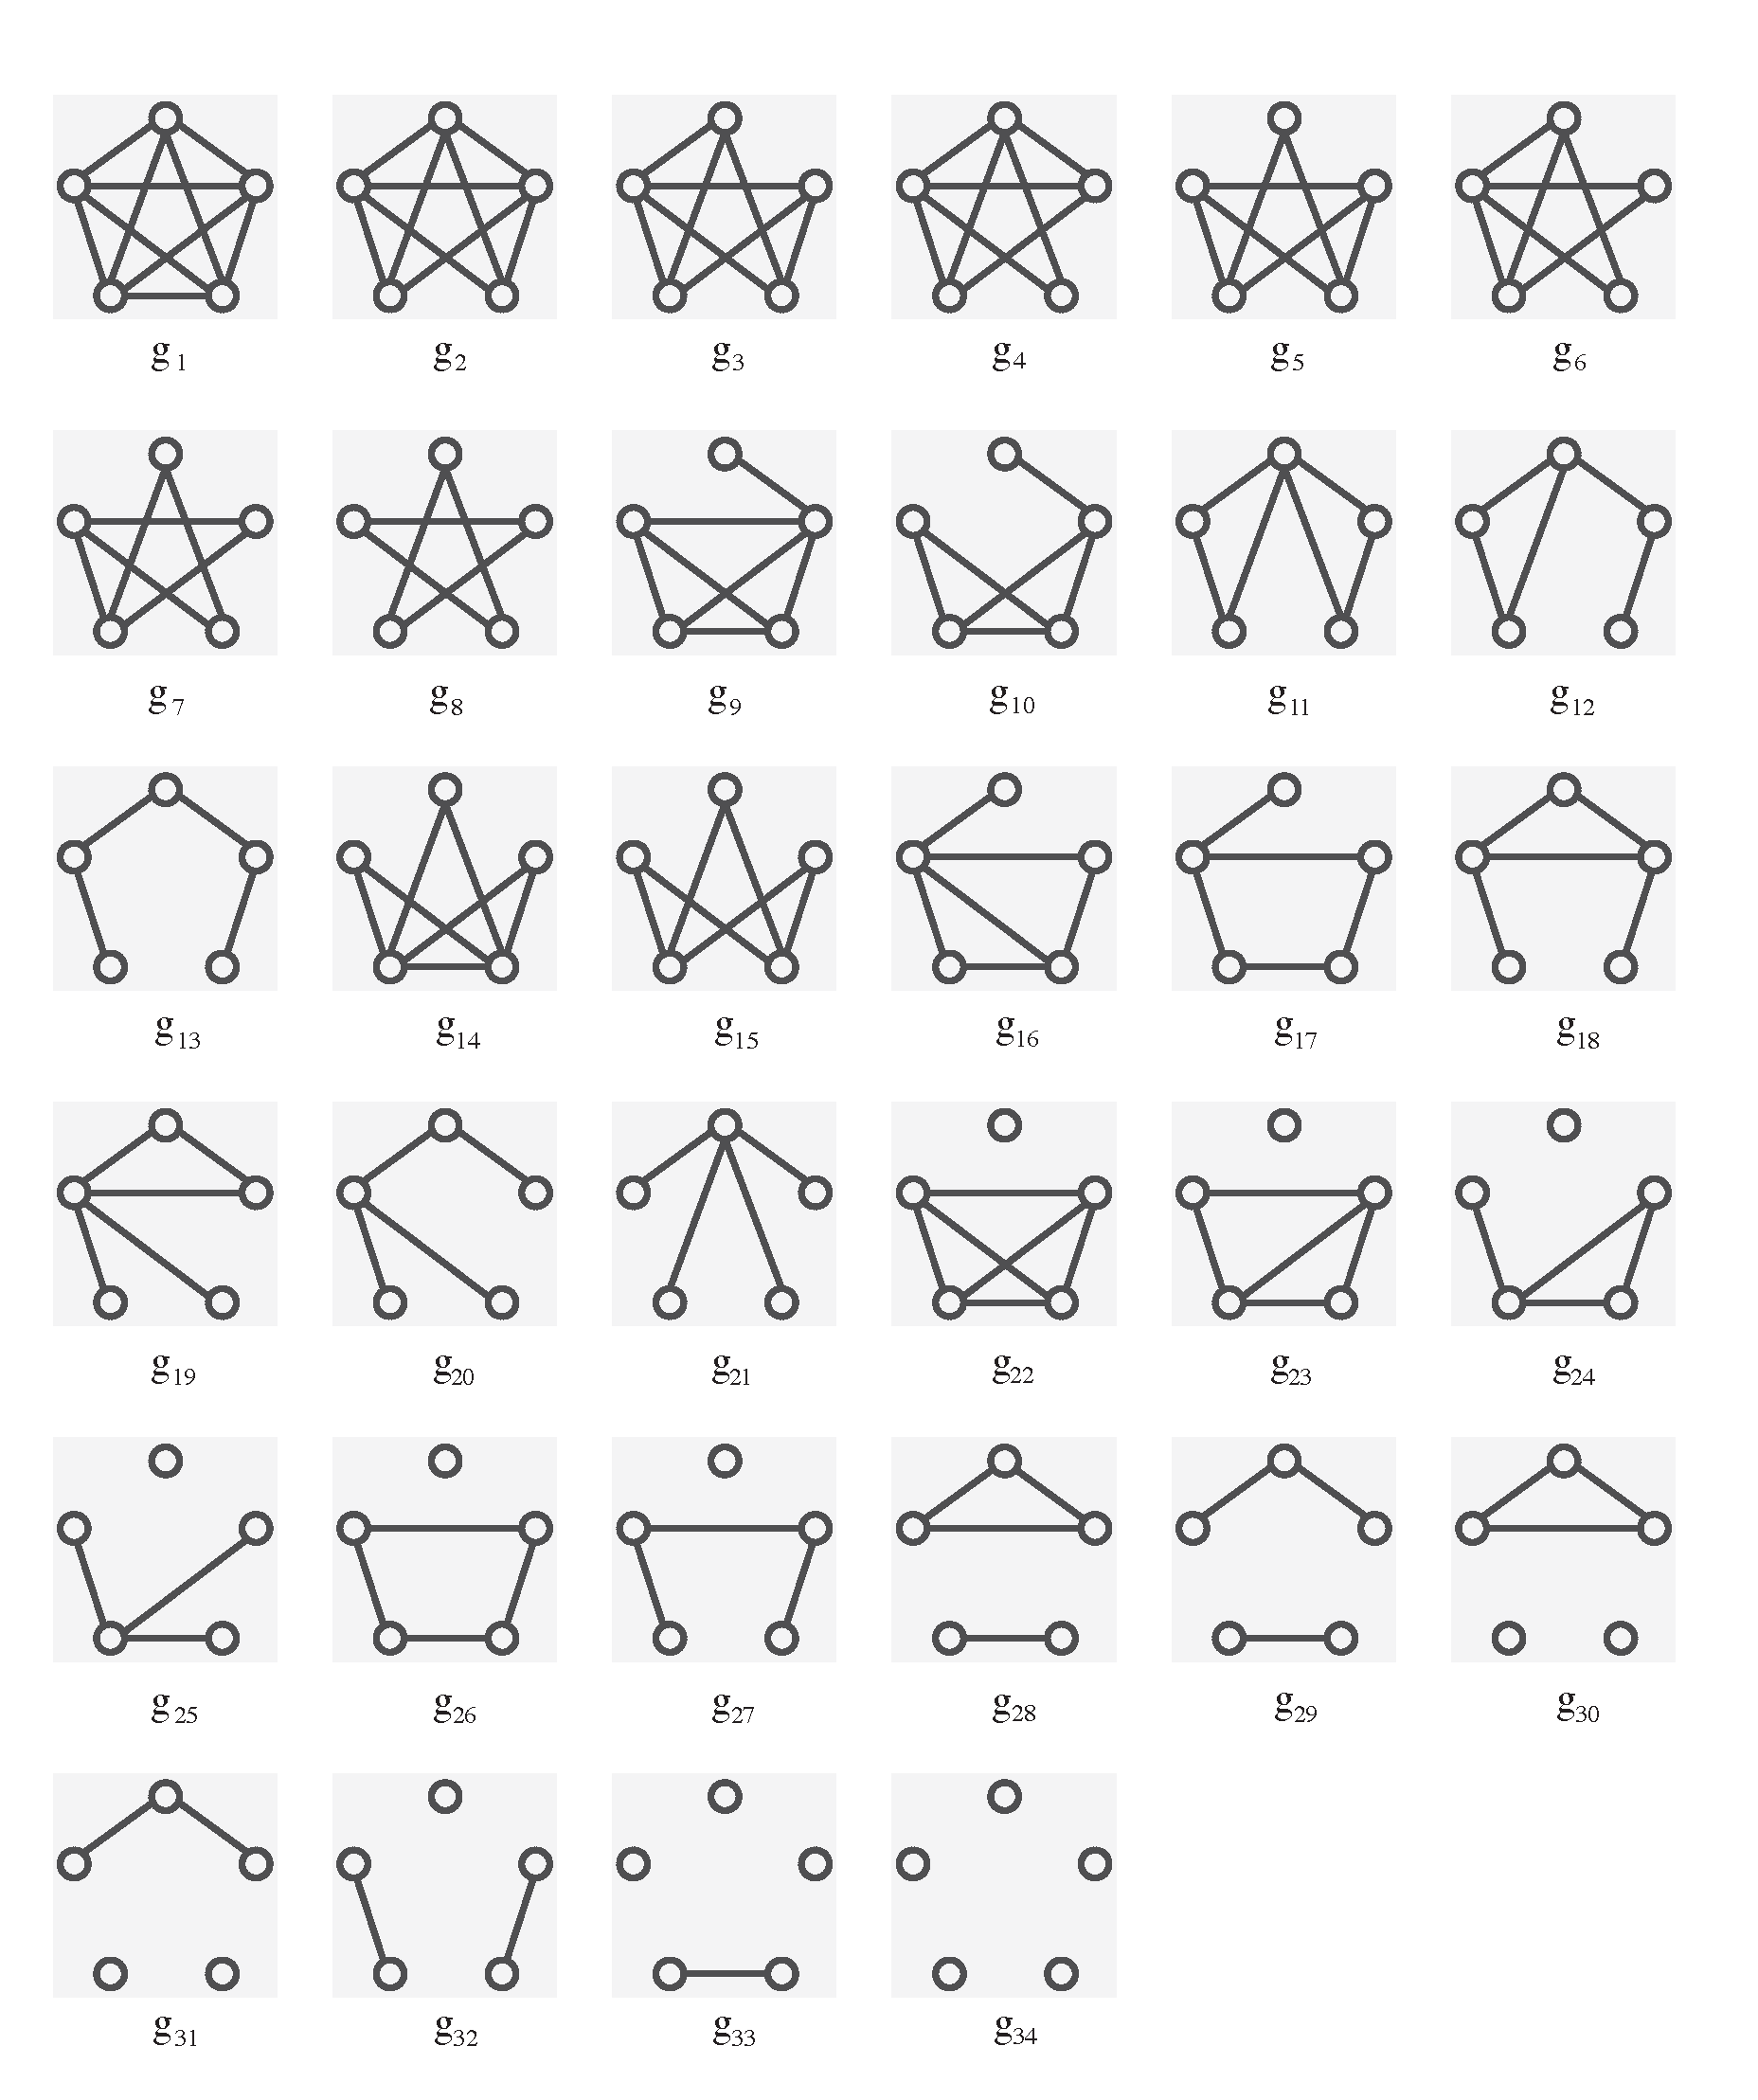
\includegraphics[width =\linewidth]{5graphlets.pdf}
\caption{Graphlets der Gr\"o"se 5 (\textit{Shervashidze et al.})}
\label{fig:5graphlets}
\end{figure}

\newpage

%TODO: UML Diagramm so, konvertieren, dass es eine Bounding Box hat und wieder einf\"ugen

\section{Tabellenverzeichnis}

\newpage


\begin{sidewaystable}

\definecolor{fGreen}{rgb}{0.13,0.54,0.13}

\scalebox{0.8}{
\begin{tabular}[h!]{l l l l l l l l l l l l l l l l l l l l l l l l}

PDB-ID & \cellcolor{fGreen!100}2utg & 1vib & 1qpu & 1qq3 & 2xl6 & 2yl1 & 1rxq & 2qe9 & 2rd9 & 1m4r & 1hgu & 1pv6 & 1awr & 1d9c & 1ngl & 1n7v & 7tim & 1ney & 1v3z & 1a17 & 1ar0 & 2v5l &  \\
2utg &   X   & 8.915 & 8.626 & 8.150 & 9.759 & 13.62 & 6.408 & 8.128 & 7.384 & 5.158 & 4.944 & 3.570 & 11.67 & 4.392 & 7.387 & 13.02 & 9.171 & 8.737 & 8.025 & 2.490 & 9.329 & 6.253 &  \\
1vib & 8.915 &   X   & 15.54 & 15.89 & 16.89 & 21.08 & 15.22 & 16.80 & 16.23 & 13.39 & 13.26 & 12.32 & 17.13 & 12.55 & 11.80 & 17.87 & 17.44 & 17.07 & 13.78 & 7.943 & 16.33 & 14.27 &  \\
1qpu & 8.626 & 15.54 &   X   & 1.451 & 3.655 & 5.632 & 6.272 & 8.187 & 7.539 & 5.410 & 7.849 & 7.087 & 11.01 & 7.053 & 9.864 & 12.54 & 8.261 & 8.829 & 8.822 & 9.192 & 9.692 & 6.462 &  \\
1qq3 & 8.150 & 15.89 & 1.451 &   X   & 3.614 & 5.651 & 6.064 & 7.554 & 7.252 & 5.087 & 7.413 & 6.776 & 11.02 & 6.721 & 9.918 & 12.56 & 7.787 & 8.354 & 8.892 & 9.531 & 9.216 & 6.019 &  \\
2xl6 & 9.759 & 16.89 & 3.655 & 3.614 &   X   & 4.518 & 5.106 & 5.523 & 5.482 & 5.514 & 8.147 & 8.655 & 8.374 & 6.685 & 8.091 & 9.919 & 5.950 & 6.459 & 6.255 & 10.30 & 7.054 & 4.716 &  \\
2yl1 & 13.62 & 21.08 & 5.632 & 5.651 & 4.518 &   X   & 7.737 & 7.197 & 7.589 & 8.855 & 11.36 & 11.82 & 11.53 & 10.34 & 12.29 & 12.94 & 8.343 & 8.923 & 10.59 & 14.75 & 10.14 & 8.137 &  \\
1rxq & 6.408 & 15.22 & 6.272 & 6.064 & 5.106 & 7.737 &   X   & 2.271 & 1.563 & 1.846 & 4.457 & 4.428 & 8.105 & 2.685 & 6.737 & 10.11 & 4.059 & 4.769 & 5.299 & 8.066 & 5.910 & 3.043 &  \\
2qe9 & 8.128 & 16.80 & 8.187 & 7.554 & 5.523 & 7.197 & 2.271 &   X   & 2.024 & 4.006 & 6.167 & 5.959 & 8.708 & 4.649 & 8.068 & 10.83 & 4.470 & 5.180 & 6.065 & 9.575 & 6.728 & 4.542 &  \\
2rd9 & 7.384 & 16.23 & 7.539 & 7.252 & 5.482 & 7.589 & 1.563 & 2.024 &   X   & 3.205 & 5.325 & 5.829 & 7.137 & 3.853 & 6.677 & 9.126 & 3.049 & 3.785 & 4.747 & 9.046 & 5.086 & 3.123 &  \\
1m4r & 5.158 & 13.39 & 5.410 & 5.087 & 5.514 & 8.855 & 1.846 & 4.006 & 3.205 &   X   & 3.657 & 3.784 & 8.468 & 1.837 & 6.243 & 10.41 & 5.063 & 5.650 & 5.068 & 6.336 & 5.972 & 2.922 &  \\
1hgu & 4.944 & 13.26 & 7.849 & 7.413 & 8.147 & 11.36 & 4.457 & 6.167 & 5.325 & 3.657 &   X   & 4.692 & 9.337 & 3.187 & 5.776 & 10.59 & 6.059 & 5.603 & 6.003 & 7.045 & 6.636 & 3.742 &  \\
1pv6 & 3.570 & 12.32 & 7.087 & 6.776 & 8.655 & 11.82 & 4.428 & 5.959 & 5.829 & 3.784 & 4.692 &   X   & 12.09 & 4.568 & 8.081 & 13.67 & 7.678 & 8.304 & 8.510 & 4.926 & 9.202 & 5.753 &  \\
1awr & 11.67 & 17.13 & 11.01 & 11.02 & 8.374 & 11.53 & 8.105 & 8.708 & 7.137 & 8.468 & 9.337 & 12.09 &   X   & 7.762 & 7.577 & 2.196 & 4.751 & 4.070 & 3.972 & 11.87 & 3.395 & 6.506 &  \\
1d9c & 4.392 & 12.55 & 7.053 & 6.721 & 6.685 & 10.34 & 2.685 & 4.649 & 3.853 & 1.837 & 3.187 & 4.568 & 7.762 &   X   & 6.366 & 9.743 & 5.605 & 5.246 & 4.468 & 5.626 & 6.116 & 3.637 &  \\
1ngl & 7.387 & 11.80 & 9.864 & 9.918 & 8.091 & 12.29 & 6.737 & 8.068 & 6.677 & 6.243 & 5.776 & 8.081 & 7.577 & 6.366 &   X   & 8.064 & 6.805 & 6.711 & 4.658 & 8.473 & 5.325 & 4.582 &  \\
1n7v & 13.02 & 17.87 & 12.54 & 12.56 & 9.919 & 12.94 & 10.11 & 10.83 & 9.126 & 10.41 & 10.59 & 13.67 & 2.196 & 9.743 & 8.064 &   X   & 6.405 & 5.675 & 5.484 & 13.53 & 4.509 & 7.987 &  \\
7tim & 9.171 & 17.44 & 8.261 & 7.787 & 5.950 & 8.343 & 4.059 & 4.470 & 3.049 & 5.063 & 6.059 & 7.678 & 4.751 & 5.605 & 6.805 & 6.405 &   X   & 0.919 & 3.869 & 11.02 & 2.858 & 3.619 &  \\
1ney & 8.737 & 17.07 & 8.829 & 8.354 & 6.459 & 8.923 & 4.769 & 5.180 & 3.785 & 5.650 & 5.603 & 8.304 & 4.070 & 5.246 & 6.711 & 5.675 & 0.919 &   X   & 3.500 & 10.59 & 2.683 & 3.646 &  \\
1v3z & 8.025 & 13.78 & 8.822 & 8.892 & 6.255 & 10.59 & 5.299 & 6.065 & 4.747 & 5.068 & 6.003 & 8.510 & 3.972 & 4.468 & 4.658 & 5.484 & 3.869 & 3.500 &   X   & 8.286 & 2.693 & 3.435 &  \\
1a17 & 2.490 & 7.943 & 9.192 & 9.531 & 10.30 & 14.75 & 8.066 & 9.575 & 9.046 & 6.336 & 7.045 & 4.926 & 11.87 & 5.626 & 8.473 & 13.53 & 11.02 & 10.59 & 8.286 &   X   & 10.56 & 7.612 &  \\
1ar0 & 9.329 & 16.33 & 9.692 & 9.216 & 7.054 & 10.14 & 5.910 & 6.728 & 5.086 & 5.972 & 6.636 & 9.202 & 3.395 & 6.116 & 5.325 & 4.509 & 2.858 & 2.683 & 2.693 & 10.56 &   X   & 3.679 &  \\
2v5l & 6.253 & 14.27 & 6.462 & 6.019 & 4.716 & 8.137 & 3.043 & 4.542 & 3.123 & 2.922 & 3.742 & 5.753 & 6.506 & 3.637 & 4.582 & 7.987 & 3.619 & 3.646 & 3.435 & 7.612 & 3.679 &   X   &  \\


\end{tabular}}

\end{sidewaystable}
\newpage




\begin{table}
\label{table:occ-aag-rgf}
\scalebox{0.8}{
\begin{tabular}{l l l l l l l l l l l l l l l l l}

PDB-ID & 1qpu & 1qq3 & 1cgn & 1he9 & 3gf9 & 1exs & 1ngl & 1qqs & 3slo & 1wjx & 5chy & 2id9 & 3i42 & 1d4o & 2w0i &  \\
1qpu &   X   & \cellcolor{fGreen!100}1.139 & \cellcolor{fGreen!75}1.296 & 6.159 & \cellcolor{fGreen!50}5.656 & 10.52 & 11.00 & 12.35 & 12.45 & 11.66 & 7.517 & \cellcolor{fGreen!25}6.128 & 6.625 & 7.326 & 8.572 &  \\
1qq3 & \cellcolor{fGreen!100}1.139 &   X   & \cellcolor{fGreen!75}1.310 & 5.980 & \cellcolor{fGreen!50}5.645 & 9.964 & 10.38 & 11.61 & 11.84 & 11.10 & 6.967 & \cellcolor{fGreen!25}5.776 & 6.039 & 7.491 & 8.059 &  \\
1cgn & \cellcolor{fGreen!100}1.296 & \cellcolor{fGreen!75}1.310 &   X   & 6.093 & \cellcolor{fGreen!25}5.737 & 9.987 & 10.44 & 11.55 & 11.81 & 11.16 & 6.801 & \cellcolor{fGreen!50}5.663 & 5.929 & 7.091 & 7.918 &  \\
1he9 & 6.159 & 5.980 & 6.093 &   X   & \cellcolor{fGreen!100}2.289 & 8.032 & 6.813 & 11.03 & 10.87 & 8.405 & \cellcolor{fGreen!25}3.974 & \cellcolor{fGreen!75}2.445 & \cellcolor{fGreen!50}3.452 & 10.93 & 4.807 &  \\
3gf9 & 5.656 & 5.645 & 5.737 & \cellcolor{fGreen!100}2.289 &   X   & 9.544 & 8.479 & 12.36 & 12.19 & 10.03 & \cellcolor{fGreen!25}5.135 & \cellcolor{fGreen!75}3.370 & \cellcolor{fGreen!50}4.359 & 12.08 & 6.018 &  \\
1exs & 10.52 & 9.964 & 9.987 & 8.032 & 9.544 &   X   & \cellcolor{fGreen!25}4.463 & \cellcolor{fGreen!50}4.041 & \cellcolor{fGreen!75}3.138 & \cellcolor{fGreen!100}2.802 & 4.773 & 7.086 & 5.541 & 7.374 & 4.530 &  \\
1ngl & 11.00 & 10.38 & 10.44 & 6.813 & 8.479 & \cellcolor{fGreen!50}4.463 &   X   & 7.716 & 6.865 & \cellcolor{fGreen!100}3.764 & \cellcolor{fGreen!25}4.718 & 6.054 & 5.065 & 9.755 & \cellcolor{fGreen!75}4.031 &  \\
1qqs & 12.35 & 11.61 & 11.55 & 11.03 & 12.36 & \cellcolor{fGreen!75}4.041 & 7.716 &   X   & \cellcolor{fGreen!100}1.674 & \cellcolor{fGreen!50}5.340 & 8.148 & 10.20 & 8.612 & \cellcolor{fGreen!25}7.226 & 7.404 &  \\
3slo & 12.45 & 11.84 & 11.81 & 10.87 & 12.19 & \cellcolor{fGreen!75}3.138 & \cellcolor{fGreen!25}6.865 & \cellcolor{fGreen!100}1.674 &   X   & \cellcolor{fGreen!50}4.750 & 7.488 & 9.994 & 8.600 & 7.680 & 6.997 &  \\
1wjx & 11.66 & 11.10 & 11.16 & 8.405 & 10.03 & \cellcolor{fGreen!100}2.802 & \cellcolor{fGreen!75}3.764 & 5.340 & \cellcolor{fGreen!25}4.750 &   X   & 5.264 & 7.522 & 5.699 & 8.450 & \cellcolor{fGreen!50}4.384 &  \\
5chy & 7.517 & 6.967 & 6.801 & \cellcolor{fGreen!25}3.974 & 5.135 & 4.773 & 4.718 & 8.148 & 7.488 & 5.264 &   X   & \cellcolor{fGreen!75}2.600 & \cellcolor{fGreen!50}2.817 & 8.667 & \cellcolor{fGreen!100}1.497 &  \\
2id9 & 6.128 & 5.776 & 5.663 & \cellcolor{fGreen!100}2.445 & \cellcolor{fGreen!25}3.370 & 7.086 & 6.054 & 10.20 & 9.994 & 7.522 & \cellcolor{fGreen!50}2.600 &   X   & \cellcolor{fGreen!75}2.447 & 10.24 & 3.657 &  \\
3i42 & 6.625 & 6.039 & 5.929 & \cellcolor{fGreen!25}3.452 & 4.359 & 5.541 & 5.065 & 8.612 & 8.600 & 5.699 & \cellcolor{fGreen!75}2.817 & \cellcolor{fGreen!100}2.447 &   X   & 9.544 & \cellcolor{fGreen!50}2.817 &  \\
1d4o & \cellcolor{fGreen!50}7.326 & 7.491 & \cellcolor{fGreen!100}7.091 & 10.93 & 12.08 & \cellcolor{fGreen!25}7.374 & 9.755 & \cellcolor{fGreen!75}7.226 & 7.680 & 8.450 & 8.667 & 10.24 & 9.544 &   X   & 8.970 &  \\
2w0i & 8.572 & 8.059 & 7.918 & 4.807 & 6.018 & 4.530 & \cellcolor{fGreen!25}4.031 & 7.404 & 6.997 & 4.384 & \cellcolor{fGreen!100}1.497 & \cellcolor{fGreen!50}3.657 & \cellcolor{fGreen!75}2.817 & 8.970 &   X   &  \\



\end{tabular}}
\caption{Distanzen der Aminos\"auregraphen, gemessen mit RGF. In den Zellen der Tabelle stehen die RGF-Distanzen f\"ur die entsprechenden PDB-Dateien. F\"ur jede Zeile (jedes Protein) sind die 4 niedrigsten Distanzen gr\"un unterlegt. Je dunkler das gr\"un ist, desto k\"urzer ist die Distanz}
\end{table}



\begin{table}
\label{table:occ-pg-rgf}
\scalebox{0.8}{
\begin{tabular}{l l l l l l l l l l l l l l l l l}


PDB-ID & 1qpu & 1qq3 & 1cgn & 1he9 & 3gf9 & 1exs & 1ngl & 1qqs & 3slo & 1wjx & 5chy & 2id9 & 3i42 & 1d4o & 2w0i &  \\
1qpu &   X   & \cellcolor{fGreen!25}0.806 & \cellcolor{fGreen!100}0.606 & \cellcolor{fGreen!50}0.697 & 3.131 & 1.159 & 2.195 & 2.197 & 1.226 & 1.049 & 1.014 & 0.811 & 1.098 & \cellcolor{fGreen!75}0.628 & 0.972 &  \\
1qq3 & \cellcolor{fGreen!25}0.806 &   X   & \cellcolor{fGreen!100}0.405 & 1.504 & 1.567 & 1.703 & 0.883 & 0.883 & 1.396 & 1.270 & 0.869 & \cellcolor{fGreen!75}0.405 & \cellcolor{fGreen!50}0.693 & 0.988 & 1.779 &  \\
1cgn & \cellcolor{fGreen!75}0.606 & \cellcolor{fGreen!100}0.405 &   X   & \cellcolor{fGreen!50}0.810 & 1.432 & 1.633 & 1.193 & 1.193 & 1.513 & 1.339 & 1.060 & \cellcolor{fGreen!25}0.811 & 1.098 & 1.011 & 1.516 &  \\
1he9 & \cellcolor{fGreen!100}0.697 & 1.504 & \cellcolor{fGreen!75}0.810 &   X   & 4.492 & 3.253 & 1.386 & 1.386 & 4.357 & 1.291 & \cellcolor{fGreen!25}1.135 & \cellcolor{fGreen!50}1.099 & 1.386 & 3.599 & 2.506 &  \\
3gf9 & 3.131 & \cellcolor{fGreen!75}1.567 & \cellcolor{fGreen!100}1.432 & 4.492 &   X   & 2.523 & 2.815 & 2.817 & \cellcolor{fGreen!50}1.596 & 2.056 & \cellcolor{fGreen!25}1.816 & 1.917 & 2.034 & 3.122 & 4.130 &  \\
1exs & \cellcolor{fGreen!50}1.159 & 1.703 & 1.633 & 3.253 & 2.523 &   X   & \cellcolor{fGreen!25}1.324 & 1.324 & 2.968 & \cellcolor{fGreen!100}0.696 & \cellcolor{fGreen!75}0.885 & 1.492 & 1.610 & 3.102 & 3.820 &  \\
1ngl & 2.195 & 0.883 & 1.193 & 1.386 & 2.815 & 1.324 &   X   & \cellcolor{fGreen!100}0.002 & \cellcolor{fGreen!50}0.787 & 2.629 & 2.279 & \cellcolor{fGreen!25}0.788 & \cellcolor{fGreen!75}0.286 & 0.980 & 2.722 &  \\
1qqs & 2.197 & 0.883 & 1.193 & 1.386 & 2.817 & 1.324 & \cellcolor{fGreen!100}0.002 &   X   & \cellcolor{fGreen!50}0.787 & 2.631 & 2.281 & \cellcolor{fGreen!25}0.788 & \cellcolor{fGreen!75}0.285 & 0.980 & 2.722 &  \\
3slo & 1.226 & 1.396 & 1.513 & 4.357 & 1.596 & 2.968 & \cellcolor{fGreen!50}0.787 & \cellcolor{fGreen!25}0.787 &   X   & \cellcolor{fGreen!100}0.257 & \cellcolor{fGreen!75}0.705 & 1.024 & 1.073 & 3.137 & 6.154 &  \\
1wjx & 1.049 & 1.270 & 1.339 & 1.291 & 2.056 & \cellcolor{fGreen!50}0.696 & 2.629 & 2.631 & \cellcolor{fGreen!100}0.257 &   X   & 1.043 & 0.933 & \cellcolor{fGreen!25}0.914 & \cellcolor{fGreen!75}0.644 & 2.093 &  \\
5chy & 1.014 & 0.869 & 1.060 & 1.135 & 1.816 & 0.885 & 2.279 & 2.281 & \cellcolor{fGreen!50}0.705 & 1.043 &   X   & \cellcolor{fGreen!75}0.607 & \cellcolor{fGreen!25}0.800 & \cellcolor{fGreen!100}0.275 & 2.282 &  \\
2id9 & 0.811 & \cellcolor{fGreen!100}0.405 & 0.811 & 1.099 & 1.917 & 1.492 & 0.788 & 0.788 & 1.024 & 0.933 & \cellcolor{fGreen!75}0.607 &   X   & \cellcolor{fGreen!50}0.692 & \cellcolor{fGreen!25}0.783 & 2.890 &  \\
3i42 & 1.098 & \cellcolor{fGreen!25}0.693 & 1.098 & 1.386 & 2.034 & 1.610 & \cellcolor{fGreen!75}0.286 & \cellcolor{fGreen!100}0.285 & 1.073 & 0.914 & 0.800 & \cellcolor{fGreen!50}0.692 &   X   & 1.076 & 3.008 &  \\
1d4o & \cellcolor{fGreen!75}0.628 & 0.988 & 1.011 & 3.599 & 3.122 & 3.102 & 0.980 & 0.980 & 3.137 & \cellcolor{fGreen!50}0.644 & \cellcolor{fGreen!100}0.275 & \cellcolor{fGreen!25}0.783 & 1.076 &   X   & 4.406 &  \\
2w0i & \cellcolor{fGreen!100}0.972 & \cellcolor{fGreen!50}1.779 & \cellcolor{fGreen!75}1.516 & 2.506 & 4.130 & 3.820 & 2.722 & 2.722 & 6.154 & \cellcolor{fGreen!25}2.093 & 2.282 & 2.890 & 3.008 & 4.406 &   X   &  \\


\end{tabular}}
\caption{Distanzen der Proteingraphen, gemessen mit RGF. In den Zellen der Tabelle stehen die RGF-Distanzen f\"ur die entsprechenden PDB-Dateien. F\"ur jede Zeile (jedes Protein) sind die 4 niedrigsten Distanzen gr\"un unterlegt. Je dunkler das gr\"un ist, desto k\"urzer ist die Distanz}
\end{table}


\begin{table}
\label{table:occ-cg-rgf}
\scalebox{0.8}{
\begin{tabular}{l l l l l l l l l l l l l l l l l}

PDB-ID & 1qpu & 1qq3 & 1cgn & 1he9 & 3gf9 & 1exs & 1ngl & 1qqs & 3slo & 1wjx & 5chy & 2id9 & 3i42 & 1d4o & 2w0i &  \\
1qpu &   X   & 4.405 & 5.056 & 2.271 & 10.75 & 3.567 & 2.309 & 13.66 & 14.10 & \cellcolor{fGreen!50}2.128 & \cellcolor{fGreen!75}1.933 & \cellcolor{fGreen!25}2.165 & \cellcolor{fGreen!100}1.877 & 8.791 & 4.422 &  \\
1qq3 & 4.405 &   X   & \cellcolor{fGreen!75}1.906 & \cellcolor{fGreen!100}1.714 & 10.03 & 3.860 & 3.457 & 6.851 & 12.70 & 2.587 & \cellcolor{fGreen!25}2.431 & 2.557 & \cellcolor{fGreen!50}2.269 & 7.907 & 3.002 &  \\
1cgn & 5.056 & 1.906 &   X   & \cellcolor{fGreen!25}0.985 & 9.469 & 1.712 & 1.979 & 7.333 & 12.20 & 1.954 & 1.120 & \cellcolor{fGreen!75}0.249 & \cellcolor{fGreen!100}0.037 & 6.501 & \cellcolor{fGreen!50}0.980 &  \\
1he9 & 2.271 & 1.714 & \cellcolor{fGreen!100}0.985 &   X   & 5.881 & 3.456 & \cellcolor{fGreen!25}1.386 & 4.069 & 5.432 & 1.466 & \cellcolor{fGreen!50}1.291 & \cellcolor{fGreen!75}1.099 & 1.386 & 9.950 & 2.506 &  \\
3gf9 & 10.75 & 10.03 & 9.469 & 5.881 &   X   & 5.473 & 4.230 & 14.86 & 15.99 & \cellcolor{fGreen!75}2.516 & \cellcolor{fGreen!100}1.971 & \cellcolor{fGreen!50}2.575 & \cellcolor{fGreen!25}2.693 & 8.811 & 11.61 &  \\
1exs & 3.567 & 3.860 & 1.712 & 3.456 & 5.473 &   X   & \cellcolor{fGreen!50}1.290 & 3.217 & 4.391 & \cellcolor{fGreen!100}0.611 & \cellcolor{fGreen!75}0.662 & \cellcolor{fGreen!25}1.459 & 1.576 & 9.191 & 4.226 &  \\
1ngl & 2.309 & 3.457 & 1.979 & \cellcolor{fGreen!25}1.386 & 4.230 & \cellcolor{fGreen!50}1.290 &   X   & 3.637 & 2.620 & 2.697 & 2.644 & \cellcolor{fGreen!75}0.788 & \cellcolor{fGreen!100}0.286 & 4.373 & 2.722 &  \\
1qqs & 13.66 & 6.851 & 7.333 & 4.069 & 14.86 & \cellcolor{fGreen!100}3.217 & \cellcolor{fGreen!25}3.637 &   X   & 12.90 & 5.645 & 4.202 & \cellcolor{fGreen!75}3.394 & \cellcolor{fGreen!50}3.512 & 16.22 & 4.907 &  \\
3slo & 14.10 & 12.70 & 12.20 & 5.432 & 15.99 & 4.391 & \cellcolor{fGreen!50}2.620 & 12.90 &   X   & 4.974 & \cellcolor{fGreen!25}3.863 & \cellcolor{fGreen!100}2.351 & \cellcolor{fGreen!75}2.412 & 14.09 & 7.116 &  \\
1wjx & 2.128 & 2.587 & 1.954 & 1.466 & 2.516 & \cellcolor{fGreen!75}0.611 & 2.697 & 5.645 & 4.974 &   X   & \cellcolor{fGreen!100}0.360 & \cellcolor{fGreen!50}0.961 & \cellcolor{fGreen!25}0.965 & 2.225 & 2.042 &  \\
5chy & 1.933 & 2.431 & 1.120 & 1.291 & 1.971 & \cellcolor{fGreen!75}0.662 & 2.644 & 4.202 & 3.863 & \cellcolor{fGreen!100}0.360 &   X   & \cellcolor{fGreen!50}0.797 & \cellcolor{fGreen!25}0.914 & 1.728 & 2.093 &  \\
2id9 & 2.165 & 2.557 & \cellcolor{fGreen!100}0.249 & 1.099 & 2.575 & 1.459 & \cellcolor{fGreen!50}0.788 & 3.394 & 2.351 & 0.961 & \cellcolor{fGreen!25}0.797 &   X   & \cellcolor{fGreen!75}0.692 & 1.921 & 2.890 &  \\
3i42 & 1.877 & 2.269 & \cellcolor{fGreen!100}0.037 & 1.386 & 2.693 & 1.576 & \cellcolor{fGreen!75}0.286 & 3.512 & 2.412 & 0.965 & \cellcolor{fGreen!25}0.914 & \cellcolor{fGreen!50}0.692 &   X   & 2.039 & 3.008 &  \\
1d4o & 8.791 & 7.907 & 6.501 & 9.950 & 8.811 & 9.191 & 4.373 & 16.22 & 14.09 & \cellcolor{fGreen!25}2.225 & \cellcolor{fGreen!100}1.728 & \cellcolor{fGreen!75}1.921 & \cellcolor{fGreen!50}2.039 &   X   & 10.76 &  \\
2w0i & 4.422 & 3.002 & \cellcolor{fGreen!100}0.980 & \cellcolor{fGreen!25}2.506 & 11.61 & 4.226 & 2.722 & 4.907 & 7.116 & \cellcolor{fGreen!75}2.042 & \cellcolor{fGreen!50}2.093 & 2.890 & 3.008 & 10.76 &   X   &  \\



\end{tabular}}
\caption{Distanzen der Komplexgraphen, gemessen mit RGF. In den Zellen der Tabelle stehen die RGF-Distanzen f\"ur die entsprechenden PDB-Dateien. F\"ur jede Zeile (jedes Protein) sind die 4 niedrigsten Distanzen gr\"un unterlegt. Je dunkler das gr\"un ist, desto k\"urzer ist die Distanz}
\end{table}



\newpage

\begin{table}
\label{table:occ-aa-tc}
\scalebox{0.8}{
\begin{tabular}{l l l l l l l l l l l l l l l l l}

PDB-ID & 1qpu & 1qq3 & 1cgn & 1he9 & 3gf9 & 1exs & 1ngl & 1qqs & 3slo & 1wjx & 5chy & 2id9 & 3i42 & 1d4o & 2w0i &  \\
1qpu &   X   & \cellcolor{fGreen!75}1.0 & \cellcolor{fGreen!100}1.0 & 0.621 & \cellcolor{fGreen!25}0.666 & 0.276 & 0.25 & 0.25 & 0.224 & 0.25 & 0.538 & \cellcolor{fGreen!50}0.714 & 0.5 & 0.363 & 0.333 &  \\
1qq3 & \cellcolor{fGreen!75}1.0 &   X   & \cellcolor{fGreen!100}1.0 & 0.621 & 0.621 & 0.304 & 0.276 & 0.304 & 0.224 & 0.25 & 0.578 & \cellcolor{fGreen!50}0.666 & \cellcolor{fGreen!25}0.666 & 0.428 & 0.463 &  \\
1cgn & \cellcolor{fGreen!100}1.0 & \cellcolor{fGreen!75}1.0 &   X   & 0.621 & \cellcolor{fGreen!50}0.714 & 0.333 & 0.224 & 0.224 & 0.224 & 0.276 & 0.5 & \cellcolor{fGreen!25}0.666 & 0.578 & 0.333 & 0.428 &  \\
1he9 & 0.621 & 0.621 & 0.621 &   X   & \cellcolor{fGreen!100}0.935 & 0.463 & 0.428 & 0.176 & 0.276 & 0.304 & \cellcolor{fGreen!25}0.621 & \cellcolor{fGreen!75}0.875 & \cellcolor{fGreen!50}0.764 & 0.333 & 0.463 &  \\
3gf9 & \cellcolor{fGreen!25}0.666 & 0.621 & \cellcolor{fGreen!50}0.714 & \cellcolor{fGreen!100}0.935 &   X   & 0.276 & 0.333 & 0.2 & 0.2 & 0.224 & 0.621 & \cellcolor{fGreen!75}0.764 & 0.621 & 0.25 & 0.463 &  \\
1exs & 0.276 & 0.304 & 0.333 & 0.463 & 0.276 &   X   & 0.621 & 0.621 & \cellcolor{fGreen!50}0.764 & \cellcolor{fGreen!100}0.875 & \cellcolor{fGreen!25}0.666 & 0.5 & 0.578 & 0.463 & \cellcolor{fGreen!75}0.818 &  \\
1ngl & 0.25 & 0.276 & 0.224 & 0.428 & 0.333 & \cellcolor{fGreen!50}0.621 &   X   & 0.276 & 0.428 & \cellcolor{fGreen!75}0.666 & \cellcolor{fGreen!25}0.621 & 0.538 & 0.578 & 0.463 & \cellcolor{fGreen!100}0.666 &  \\
1qqs & 0.25 & 0.304 & 0.224 & 0.176 & 0.2 & \cellcolor{fGreen!50}0.621 & 0.276 &   X   & \cellcolor{fGreen!100}1.0 & \cellcolor{fGreen!75}0.621 & \cellcolor{fGreen!25}0.5 & 0.276 & 0.395 & 0.463 & 0.463 &  \\
3slo & 0.224 & 0.224 & 0.224 & 0.276 & 0.2 & \cellcolor{fGreen!75}0.764 & 0.428 & \cellcolor{fGreen!100}1.0 &   X   & \cellcolor{fGreen!50}0.538 & 0.463 & 0.333 & 0.395 & 0.463 & \cellcolor{fGreen!25}0.5 &  \\
1wjx & 0.25 & 0.25 & 0.276 & 0.304 & 0.224 & \cellcolor{fGreen!100}0.875 & \cellcolor{fGreen!75}0.666 & \cellcolor{fGreen!50}0.621 & 0.538 &   X   & 0.538 & 0.363 & 0.5 & 0.395 & \cellcolor{fGreen!25}0.621 &  \\
5chy & 0.538 & 0.578 & 0.5 & 0.621 & 0.621 & \cellcolor{fGreen!25}0.666 & 0.621 & 0.5 & 0.463 & 0.538 &   X   & \cellcolor{fGreen!75}0.818 & \cellcolor{fGreen!50}0.764 & 0.428 & \cellcolor{fGreen!100}1.0 &  \\
2id9 & 0.714 & 0.666 & 0.666 & \cellcolor{fGreen!100}0.875 & \cellcolor{fGreen!25}0.764 & 0.5 & 0.538 & 0.276 & 0.333 & 0.363 & \cellcolor{fGreen!75}0.818 &   X   & \cellcolor{fGreen!50}0.818 & 0.304 & 0.621 &  \\
3i42 & 0.5 & 0.666 & 0.578 & \cellcolor{fGreen!50}0.764 & 0.621 & 0.578 & 0.578 & 0.395 & 0.395 & 0.5 & \cellcolor{fGreen!75}0.764 & \cellcolor{fGreen!100}0.818 &   X   & 0.333 & \cellcolor{fGreen!25}0.714 &  \\
1d4o & 0.363 & 0.428 & 0.333 & 0.333 & 0.25 & \cellcolor{fGreen!25}0.463 & \cellcolor{fGreen!50}0.463 & \cellcolor{fGreen!100}0.463 & \cellcolor{fGreen!75}0.463 & 0.395 & 0.428 & 0.304 & 0.333 &   X   & 0.333 &  \\
2w0i & 0.333 & 0.463 & 0.428 & 0.463 & 0.463 & \cellcolor{fGreen!75}0.818 & \cellcolor{fGreen!25}0.666 & 0.463 & 0.5 & 0.621 & \cellcolor{fGreen!100}1.0 & 0.621 & \cellcolor{fGreen!50}0.714 & 0.333 &   X   &  \\


\end{tabular}}
\caption{Jaccard-Indizes der Aminos\"auregraphen. In den Zellen der Tabelle stehen die Jaccard-Indizes f\"ur die entsprechenden PDB-Dateien. F\"ur jede Zeile (jedes Protein) sind die 4 gr\"o"sten Indizes gr\"un unterlegt. Je dunkler das gr\"un ist, desto gr\"o"ser der Index}
\end{table}

\begin{table}
\label{table:occ-pg-tf}
\scalebox{0.8}{
\begin{tabular}{l l l l l l l l l l l l l l l l l}

PDB-ID & 1qpu & 1qq3 & 1cgn & 1he9 & 3gf9 & 1exs & 1ngl & 1qqs & 3slo & 1wjx & 5chy & 2id9 & 3i42 & 1d4o & 2w0i &  \\
1qpu &   X   & \cellcolor{fGreen!75}0.764 & \cellcolor{fGreen!100}0.764 & 0.578 & 0.463 & 0.463 & 0.621 & 0.621 & 0.428 & 0.578 & 0.666 & \cellcolor{fGreen!50}0.666 & \cellcolor{fGreen!25}0.666 & 0.538 & 0.395 &  \\
1qq3 & 0.764 &   X   & \cellcolor{fGreen!100}0.935 & 0.764 & 0.463 & 0.621 & 0.714 & 0.714 & 0.538 & 0.714 & \cellcolor{fGreen!25}0.764 & \cellcolor{fGreen!75}0.875 & \cellcolor{fGreen!50}0.818 & 0.666 & 0.5 &  \\
1cgn & \cellcolor{fGreen!25}0.764 & \cellcolor{fGreen!100}0.935 &   X   & 0.764 & 0.428 & 0.578 & 0.714 & 0.714 & 0.538 & 0.666 & 0.714 & \cellcolor{fGreen!75}0.875 & \cellcolor{fGreen!50}0.818 & 0.621 & 0.463 &  \\
1he9 & 0.578 & \cellcolor{fGreen!75}0.764 & \cellcolor{fGreen!100}0.764 &   X   & 0.463 & 0.578 & 0.621 & 0.621 & 0.578 & 0.538 & 0.621 & \cellcolor{fGreen!25}0.714 & \cellcolor{fGreen!50}0.714 & 0.666 & 0.538 &  \\
3gf9 & 0.463 & 0.463 & 0.428 & 0.463 &   X   & 0.428 & \cellcolor{fGreen!25}0.463 & 0.463 & 0.463 & \cellcolor{fGreen!50}0.463 & \cellcolor{fGreen!100}0.538 & 0.428 & 0.463 & \cellcolor{fGreen!75}0.5 & 0.333 &  \\
1exs & 0.463 & \cellcolor{fGreen!25}0.621 & 0.578 & 0.578 & 0.428 &   X   & 0.5 & 0.5 & \cellcolor{fGreen!100}0.714 & 0.5 & 0.578 & \cellcolor{fGreen!50}0.666 & 0.578 & \cellcolor{fGreen!75}0.714 & 0.621 &  \\
1ngl & 0.621 & 0.714 & 0.714 & 0.621 & 0.463 & 0.5 &   X   & \cellcolor{fGreen!100}1.0 & 0.538 & \cellcolor{fGreen!50}0.818 & \cellcolor{fGreen!25}0.818 & 0.818 & \cellcolor{fGreen!75}0.875 & 0.578 & 0.395 &  \\
1qqs & 0.621 & 0.714 & 0.714 & 0.621 & 0.463 & 0.5 & \cellcolor{fGreen!100}1.0 &   X   & 0.538 & \cellcolor{fGreen!25}0.818 & 0.818 & \cellcolor{fGreen!50}0.818 & \cellcolor{fGreen!75}0.875 & 0.578 & 0.395 &  \\
3slo & 0.428 & 0.538 & 0.538 & 0.578 & 0.463 & \cellcolor{fGreen!100}0.714 & 0.538 & 0.538 &   X   & 0.538 & 0.5 & \cellcolor{fGreen!25}0.578 & \cellcolor{fGreen!75}0.621 & \cellcolor{fGreen!50}0.578 & 0.463 &  \\
1wjx & 0.578 & 0.714 & 0.666 & 0.538 & 0.463 & 0.5 & \cellcolor{fGreen!50}0.818 & \cellcolor{fGreen!100}0.818 & 0.538 &   X   & \cellcolor{fGreen!25}0.764 & 0.714 & \cellcolor{fGreen!75}0.818 & 0.538 & 0.395 &  \\
5chy & 0.666 & 0.764 & 0.714 & 0.621 & 0.538 & 0.578 & \cellcolor{fGreen!75}0.818 & \cellcolor{fGreen!25}0.818 & 0.5 & 0.764 &   X   & \cellcolor{fGreen!100}0.875 & \cellcolor{fGreen!50}0.818 & 0.621 & 0.395 &  \\
2id9 & 0.666 & \cellcolor{fGreen!50}0.875 & \cellcolor{fGreen!25}0.875 & 0.714 & 0.428 & 0.666 & 0.818 & 0.818 & 0.578 & 0.714 & \cellcolor{fGreen!75}0.875 &   X   & \cellcolor{fGreen!100}0.935 & 0.714 & 0.463 &  \\
3i42 & 0.666 & 0.818 & 0.818 & 0.714 & 0.463 & 0.578 & \cellcolor{fGreen!50}0.875 & \cellcolor{fGreen!75}0.875 & 0.621 & \cellcolor{fGreen!25}0.818 & 0.818 & \cellcolor{fGreen!100}0.935 &   X   & 0.666 & 0.463 &  \\
1d4o & 0.538 & \cellcolor{fGreen!50}0.666 & 0.621 & 0.666 & 0.5 & \cellcolor{fGreen!100}0.714 & 0.578 & 0.578 & 0.578 & 0.538 & 0.621 & \cellcolor{fGreen!75}0.714 & \cellcolor{fGreen!25}0.666 &   X   & 0.5 &  \\
2w0i & 0.395 & \cellcolor{fGreen!50}0.5 & 0.463 & \cellcolor{fGreen!75}0.538 & 0.333 & \cellcolor{fGreen!100}0.621 & 0.395 & 0.395 & 0.463 & 0.395 & 0.395 & 0.463 & 0.463 & \cellcolor{fGreen!25}0.5 &   X   &  \\

\end{tabular}}
\caption{Jaccard-Indizes der Proteingraphen. In den Zellen der Tabelle stehen die Jaccard-Indizes f\"ur die entsprechenden PDB-Dateien. F\"ur jede Zeile (jedes Protein) sind die 4 gr\"o"sten Indizes gr\"un unterlegt. Je dunkler das gr\"un ist, desto gr\"o"ser der Index}
\end{table}


\begin{table}
\label{table:occ-cg-tc}
\scalebox{0.8}{
\begin{tabular}{l l l l l l l l l l l l l l l l l}

PDB-ID & 1qpu & 1qq3 & 1cgn & 1he9 & 3gf9 & 1exs & 1ngl & 1qqs & 3slo & 1wjx & 5chy & 2id9 & 3i42 & 1d4o & 2w0i &  \\
1qpu &   X   & \cellcolor{fGreen!100}0.428 & 0.395 & \cellcolor{fGreen!50}0.428 & 0.153 & 0.304 & 0.395 & 0.132 & 0.111 & 0.363 & 0.395 & \cellcolor{fGreen!75}0.428 & \cellcolor{fGreen!25}0.428 & 0.276 & 0.276 &  \\
1qq3 & 0.428 &   X   & \cellcolor{fGreen!100}0.666 & \cellcolor{fGreen!75}0.621 & 0.2 & 0.395 & 0.5 & 0.2 & 0.090 & 0.5 & 0.5 & \cellcolor{fGreen!50}0.538 & \cellcolor{fGreen!25}0.538 & 0.333 & 0.428 &  \\
1cgn & 0.395 & \cellcolor{fGreen!100}0.666 &   X   & \cellcolor{fGreen!75}0.621 & 0.224 & 0.428 & 0.5 & 0.224 & 0.111 & 0.463 & 0.5 & \cellcolor{fGreen!25}0.538 & \cellcolor{fGreen!50}0.538 & 0.363 & 0.363 &  \\
1he9 & 0.428 & 0.621 & 0.621 &   X   & 0.25 & 0.578 & \cellcolor{fGreen!50}0.621 & 0.153 & 0.090 & 0.538 & \cellcolor{fGreen!25}0.621 & \cellcolor{fGreen!100}0.714 & \cellcolor{fGreen!75}0.714 & 0.428 & 0.538 &  \\
3gf9 & 0.153 & 0.2 & 0.224 & 0.25 &   X   & \cellcolor{fGreen!75}0.276 & 0.224 & 0.153 & 0.153 & \cellcolor{fGreen!50}0.276 & \cellcolor{fGreen!100}0.304 & 0.25 & 0.224 & \cellcolor{fGreen!25}0.276 & 0.224 &  \\
1exs & 0.304 & 0.395 & 0.428 & 0.578 & 0.276 &   X   & 0.5 & 0.2 & 0.153 & \cellcolor{fGreen!25}0.578 & 0.578 & \cellcolor{fGreen!100}0.666 & \cellcolor{fGreen!50}0.578 & 0.5 & \cellcolor{fGreen!75}0.621 &  \\
1ngl & 0.395 & 0.5 & 0.5 & 0.621 & 0.224 & 0.5 &   X   & 0.132 & 0.132 & \cellcolor{fGreen!25}0.818 & \cellcolor{fGreen!75}0.818 & \cellcolor{fGreen!50}0.818 & \cellcolor{fGreen!100}0.875 & 0.428 & 0.395 &  \\
1qqs & 0.132 & \cellcolor{fGreen!50}0.2 & \cellcolor{fGreen!100}0.224 & 0.153 & 0.153 & \cellcolor{fGreen!25}0.2 & 0.132 &   X   & \cellcolor{fGreen!75}0.224 & 0.132 & 0.132 & 0.132 & 0.132 & 0.132 & 0.2 &  \\
3slo & 0.111 & 0.090 & 0.111 & 0.090 & \cellcolor{fGreen!25}0.153 & \cellcolor{fGreen!50}0.153 & 0.132 & \cellcolor{fGreen!100}0.224 &   X   & 0.111 & 0.090 & 0.090 & 0.111 & 0.111 & \cellcolor{fGreen!75}0.153 &  \\
1wjx & 0.363 & 0.5 & 0.463 & 0.538 & 0.276 & 0.578 & \cellcolor{fGreen!50}0.818 & 0.132 & 0.111 &   X   & \cellcolor{fGreen!100}0.935 & \cellcolor{fGreen!25}0.714 & \cellcolor{fGreen!75}0.818 & 0.5 & 0.395 &  \\
5chy & 0.395 & 0.5 & 0.5 & 0.621 & 0.304 & 0.578 & \cellcolor{fGreen!25}0.818 & 0.132 & 0.090 & \cellcolor{fGreen!100}0.935 &   X   & \cellcolor{fGreen!75}0.875 & \cellcolor{fGreen!50}0.818 & 0.5 & 0.395 &  \\
2id9 & 0.428 & 0.538 & 0.538 & 0.714 & 0.25 & 0.666 & \cellcolor{fGreen!50}0.818 & 0.132 & 0.090 & \cellcolor{fGreen!25}0.714 & \cellcolor{fGreen!75}0.875 &   X   & \cellcolor{fGreen!100}0.935 & 0.5 & 0.463 &  \\
3i42 & 0.428 & 0.538 & 0.538 & 0.714 & 0.224 & 0.578 & \cellcolor{fGreen!75}0.875 & 0.132 & 0.111 & \cellcolor{fGreen!25}0.818 & \cellcolor{fGreen!50}0.818 & \cellcolor{fGreen!100}0.935 &   X   & 0.428 & 0.463 &  \\
1d4o & 0.276 & 0.333 & 0.363 & 0.428 & 0.276 & \cellcolor{fGreen!100}0.5 & 0.428 & 0.132 & 0.111 & \cellcolor{fGreen!50}0.5 & \cellcolor{fGreen!25}0.5 & \cellcolor{fGreen!75}0.5 & 0.428 &   X   & 0.333 &  \\
2w0i & 0.276 & 0.428 & 0.363 & \cellcolor{fGreen!75}0.538 & 0.224 & \cellcolor{fGreen!100}0.621 & 0.395 & 0.2 & 0.153 & 0.395 & 0.395 & \cellcolor{fGreen!25}0.463 & \cellcolor{fGreen!50}0.463 & 0.333 &   X   &  \\

\end{tabular}}
\caption{Jaccard-Indizes der Komplexgraphen. In den Zellen der Tabelle stehen die Jaccard-Indizes f\"ur die entsprechenden PDB-Dateien. F\"ur jede Zeile (jedes Protein) sind die 4 gr\"o"sten Indizes gr\"un unterlegt. Je dunkler das gr\"un ist, desto gr\"o"ser der Index}
\end{table}


\begin{table}
\label{tab:correlations}
\begin{tabular}{c c c c}
Datensatz & AAG     &     PG &     CG \\
AAG       &  1      & 0.6911 & 0.7656 \\
PG        &  0.6911 &      1 & 0.6939 \\
CG        &  0.6939 & 0.6939 & 1      \\

\end{tabular}
\caption{Korrelationen der \"Ahnlichkeitsbewertungen der verschiedenen Graphformate}
\end{table}

\chapter{Schnittreste}

\section{alte Motivation}

\paragraph{Die \"Ahnlickeit} von Proteinen zu bestimmen ist eine gro"se Herausforderung. In der Zeit als wenige Strukturen bekannt waren wurde die strukturelle \"Ahnlichkeit von Proteinen noch von Experten visuell bewertet, aber mittlerweile befinden sich die Strukturen von \"uber 100000 biologischen Makromolek\"ulen in der PDB. Der Vergleich dieser gigantischen Anzahl von Strukturdaten erfordert effiziente Analysemethoden. Solche Analysen k\"onnen tiefe Einblicke in die ferne evolution\"are Verwandschaft von Proteinen liefern und sie helfen bei der Bestimmung der Funktion eines Proteins. Sie sind im Bereich des \textit{Drug-Design} hoch interessant, denn  Strukturdaten liefer Informationen \"uber m \"ogliche Liganden, die ein Protein binden kann und damit auch \"uber m\"ogliche Ziele von Medikamenten bei der Bek\"ampfung von Krankheiten. Deshalb sind strukturbasierte \"Ahnlichkeitsanalysen in der pharmakologischen Forschung von zentraler Bedeutung.
Das Problem hierbei ist, dass die Berechnung der \"Ahnlichkeit von 3D-Strukturen algorithmisch ein schwieriges Problem darstellt; lange Berechnungszeiten sind die Regel und es ist schwierig herauszufinden, ob der gefundene \"Ahnlichkeitswert f\"ur zwei Proteine nur ein lokales Optimum darstellt.
Deshalb wird versucht, von der 3D-Darstellung zu abstrahieren, ohne zentrale Strukturinformationen zu verlieren. \emph{Dali} \cite{dali}verwendet beispielsweise Distanzmatrizen, die die Abst\"ande einzelner Residuen zueinander speichern, anstatt die Koordinaten jedes Atoms abdsspzuspeichern.
Der Strukturvergleich findet dann als Vergleich dieser Distanzmatrizen statt.

Auch Graphen eignen sich, um Strukturdaten in einer leichter zu analysierenden Form abzuspeichern. Denn Graphen k\"onnen genau wie Distanzmatrizen Informationen \"uber r\"aumliche N\"ahe aufbewahren.
Die PTGL \cite{ptgl1} speichert Proteinstrukturtopologien als Graphen ab. So werden zentrale Informationen \"uber die Struktur eines Proteins aufbewahrt w\"ahrend die Gr\"o"se der Daten ma"sgeblich reduziert wird. Diese Darstellung hat den weiteren Vorteil, dass Graphen zu den meistuntersuchten mathematischen strukturen der letzten Jahre geh\"oren. Soziale Netzwerke, Interaktionen von Proteinen in Zellen, das Internet: All diese Dinge lassen sich als Graphen darstellem und werden als solche untersucht.
Doch auch die \"Ahnlichkeit von Graphen zu bestimmen ist ein schwieriges Problem. Es leitet sich vom \emph{Graph-Isomorphismus-Problem} ab. Es ist nicht klar, ob dieses Problem NP-vollst\"andig ist. In den letzten Jahren wurde \textit{Feature}-basierte Methoden erforscht, die diese Problem reduzieren. Anstatt direkt zwei Graphen miteinander zu vergleichen, werden \textit{Features} verglichen, so dass einfache Datenpunkte anstatt von komplexen Graphen verglichen werden.
Solche Methoden wurden h\"aufig erfolgreich angewandt. Diese Anwendungen fanden immer auf gro"sen Netzwerken statt. Nun stellt sich die Frage, ob sich solche Methoden auch f\"ur deutlich kleinere Netzwerke eignen. in der vorliegenden Arbeit wird eine solche \textit{Feature}-basierte Methode - der \textit{Graphlet}-Algorithmus auf verschiedene Proteingraphen angewandt. 






\bibliographystyle{plain}
\bibliography{literatur}



\end{document}